\documentclass[aspectratio=1610]{beamer}

\usetheme{KTH}
\usepackage{preamble}

% Advice from Schule, that was given to him as advice when he was becoming a researcher.
%
% Three thirds, 1 third for everybody, 1 third for experts, and 1 third for yourself to show off.

% ====>>>>> general

%% The slides should be for the audience, to give them a visual experience.
%% Transitions; one style for the slides and one style for the transitions between topics. e.g. light background, dark text vs. dark background, light text.
%% Don't write too much on the slides.
%% Skip effects.
%% Masking images to direct attention.
%% Simple charts and graphs. If possible, in the same style as the presentation (e.g. fonts, colors).

\begin{document}

% Add page numbers.
\addtobeamertemplate{navigation symbols}{}{\insertframenumber / \inserttotalframenumber}

% === [ Start page ] ===========================================================

\startpage

\begin{frame}
	\vspace{0.02\textheight}

	\begin{Large}
		Evaluation of Methods for Effective Control Flow Recovery
	\end{Large}

	\vspace{0.1\textheight}

	\begin{small}
		\textit{Robin Eklind}
	\end{small}
\end{frame}

% === [ Disposition ] ==========================================================

\normalpage

\begin{frame}
	\frametitle{Disposition}

	\begin{enumerate}
		\item What? \textit{Control Flow Recovery}
		\item Why? \textit{Applications of Control Flow Recovery}
		\item How? \textit{Control Flow Recovery Methods}
		\item Technical Contributions
		\item Future Work
		\item Demo!
	\end{enumerate}
\end{frame}


% === [ Introduction ] =========================================================

% ====>>>>> What?

% What?

% Frame problem at a high level.
% 1-3 minutes.

% Key message you wish to communicate. From the perspective of the audience, what will they gain? What can they do with the information?

\begin{frame}
	\frametitle{What?}

	\begin{block}{Control Flow Recovery}
		Analysis of control flow graphs (CFGs) to recover high-level control flow primitives (e.g. \texttt{if}-statements and \texttt{for}-loops) from assembly or low-level intermediate representations.
	\end{block}
\end{frame}

\begin{frame}
	\frametitle{Control Flow Recovery}

	\begin{figure}[htbp]
		\centering
		\begin{subfigure}[t]{0.52\textwidth}
			\centering
			\lstinputlisting[caption={LLVM IR assembly.}, language=llvm, style=nasm, basicstyle=\tiny\ttfamily, breaklines=false, numbers=none]{inc/overview/overview_mini.ll}
		\end{subfigure}
		\quad
		\begin{subfigure}[t]{0.27\textwidth}
			\centering
			\lstinputlisting[caption={C source file.}, language=C, style=c, basicstyle=\tiny\ttfamily, breaklines=false, numbers=none]{inc/overview/overview.c}
		\end{subfigure}
		\caption{\textit{Reverse compilation}, going from low-level (left) to high-level (right).}
	\end{figure}

\end{frame}

% ====>>>>> Why?

% Why?

% Then go into depth; both intellectual and emotional arguments for the severity of the problem.
% 15-20 minutes if presenting for 1 hour.

\begin{frame}
	\frametitle{Why?}

	\begin{block}{Applications of Control Flow Recovery}
		\begin{itemize}
			\item Malware analysis
			\item Security assessments
			\begin{itemize}
				\item Automated vulnerability scanning
			\end{itemize}
			\item Control-flow aware compiler passes
			\item Enable high-level data-flow analysis on IR (Rosen's method)
			\item Verification of compiler output (\textit{Reflections on Trusting Trust})
			\item Reverse compilation
			\begin{itemize}
				\item Transpilation between programming languages ($n + m$)
				\item Migrate proprietary software from legacy architectures
				\item Re-optimization of software where source code or tool chain is missing
			\end{itemize}
% Note to speaker: For Cobol.
%   - semantic equivalence, with a lot of goto-s to begin.
%   - clean up over time.
		\end{itemize}
	\end{block}
\end{frame}

\begin{frame}
	\frametitle{Control-flow Aware Compiler Passes}

	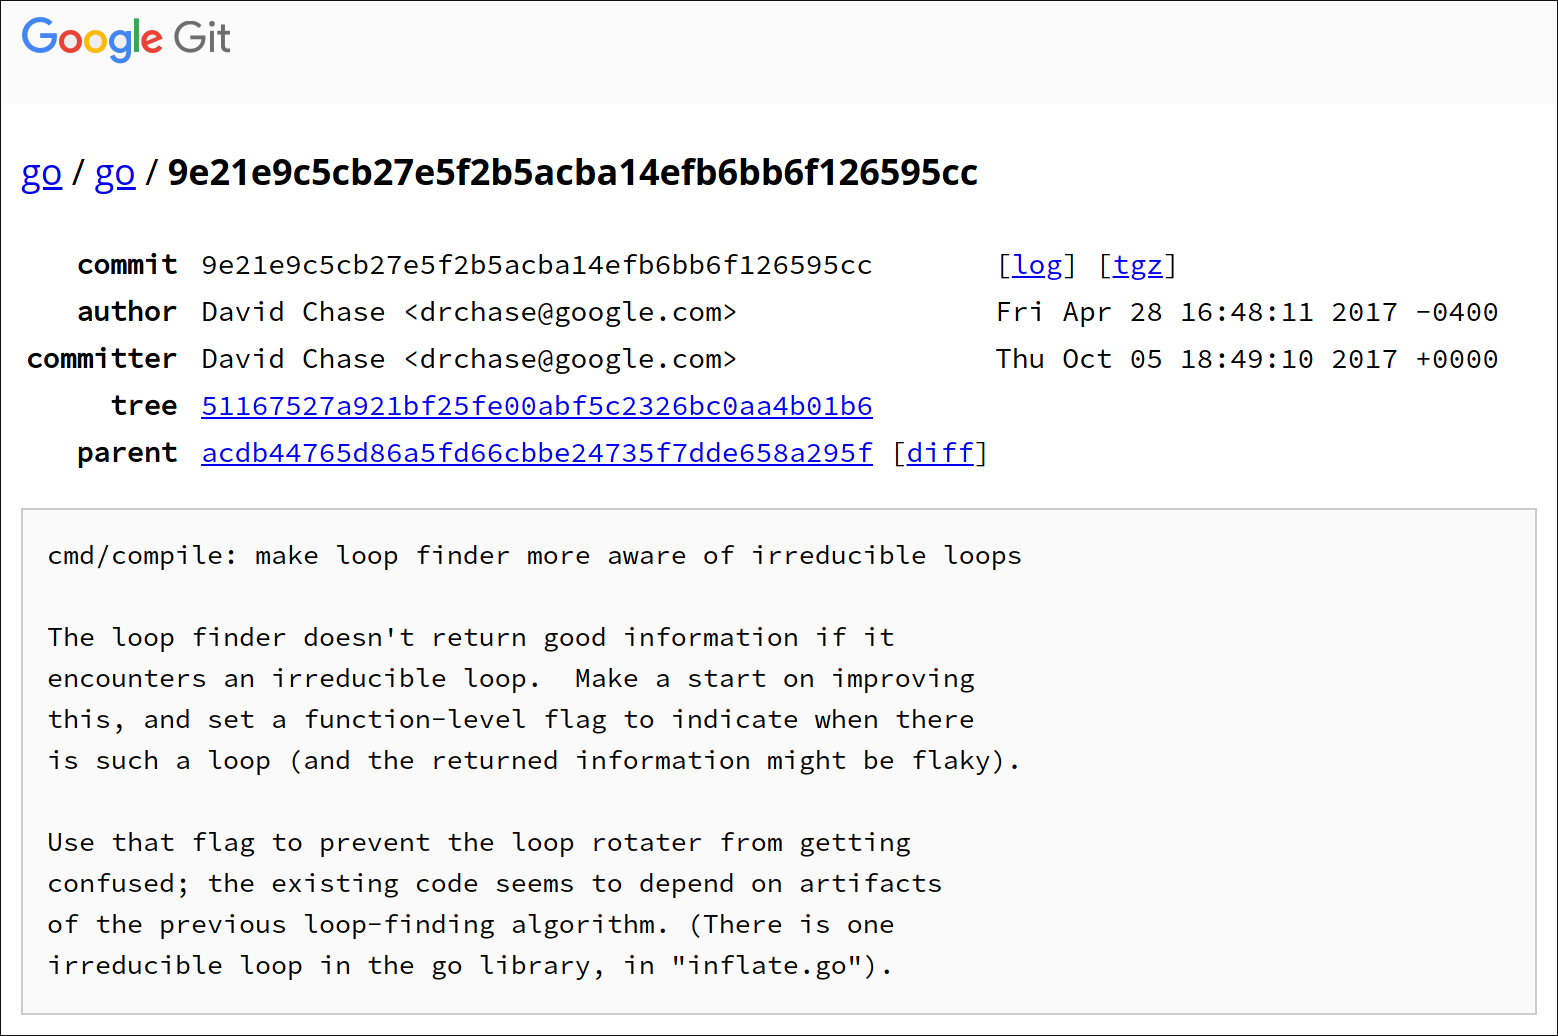
\includegraphics[width=0.8\textwidth]{inc/applications/loop_finder.png}
\end{frame}

\begin{frame}
	\frametitle{Issues with State-of-the-Art Reverse Compilation Tools}

	\begin{figure}[htbp]
		\centering
		\begin{subfigure}[ht]{0.30\textwidth}
			\centering
			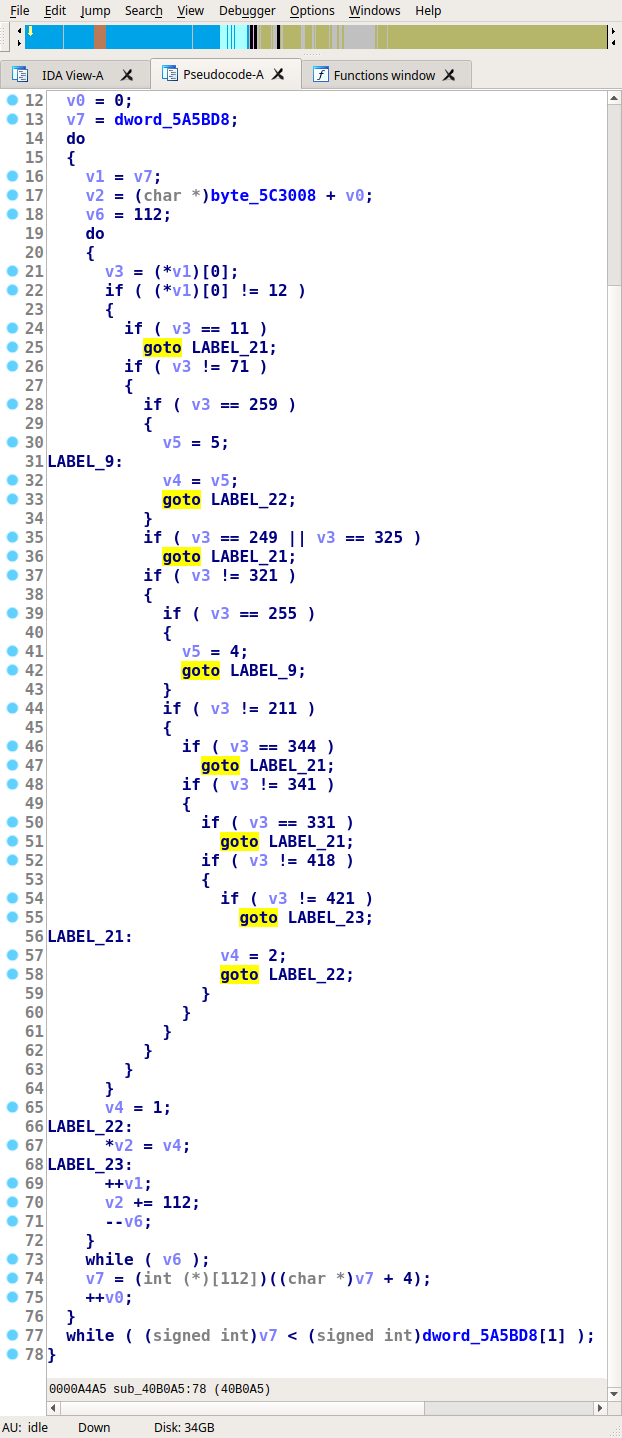
\includegraphics[height=0.80\textheight]{inc/applications/ida/ida_40B0A5.png}
		\end{subfigure}
		\begin{subfigure}[ht]{0.40\textwidth}
			\centering
			\lstinputlisting[caption={Corresponding Go source code.}, language=go, style=go, basicstyle=\tiny\ttfamily, breaklines=false, numbers=none]{inc/applications/ida/go_40B0A5.go}
		\end{subfigure}
		% IDA Version 7.1.180227
		\caption{IDA output (left) and corresponding Go source code (right).}
	\end{figure}
\end{frame}

% ====>>>>> How?

% How?

% Give solution, including benefits and drawbacks.

\begin{frame}
	\frametitle{How?}

	\begin{block}{Control Flow Recovery Methods}
		\begin{itemize}
			\item Hammock method
			\item Interval method
			\item Pattern-independent method
		\end{itemize}
	\end{block}

	There are benefits and drawbacks with each method.
\end{frame}

% --- [ Evaluation metric ] ----------------------------------------------------

\begin{frame}
	\frametitle{Evaluation metric}

	\begin{itemize}
		\item \textbf{False positive}: control flow primitive recovered but \textit{not} present in original source code.
		\item \textbf{False negative}: control flow primitive \textit{not} recovered but present in original source code.
	\end{itemize}
\end{frame}

% --- [ Hammock method ] -------------------------------------------------------

\begin{frame}
	\frametitle{Hammock method}

	Model high-level control flow primitives as subgraphs and use \textit{subgraph isomorphism search} to locate the corresponding subgraphs in CFGs.

	\vspace*{2em}

	\begin{block}{Pros}
		\begin{itemize}
			\item \textit{no} false positives
		\end{itemize}
	\end{block}

	\begin{block}{Cons}
		\begin{itemize}
			\item \textit{many} false negatives
			\item requires single-entry/single-exit invariant for subgraphs.
			%\footnote{This requirement may be relaxed to single-entry/single-successor, as detailed in 2011, Enhanced Structural Analysis for C Code Reconstruction from IR Code. F. Engel, et al.}
		\end{itemize}
	\end{block}

\end{frame}

\begin{frame}
	\frametitle{Hammock method}

	\begin{figure}[htbp]
		\centering
		\begin{subfigure}[b]{0.20\textwidth}
			\centering
			\lstinputlisting[language=C, style=c, basicstyle=\tiny\ttfamily, breaklines=false, numbers=none]{inc/methods/hammock/if.c}
			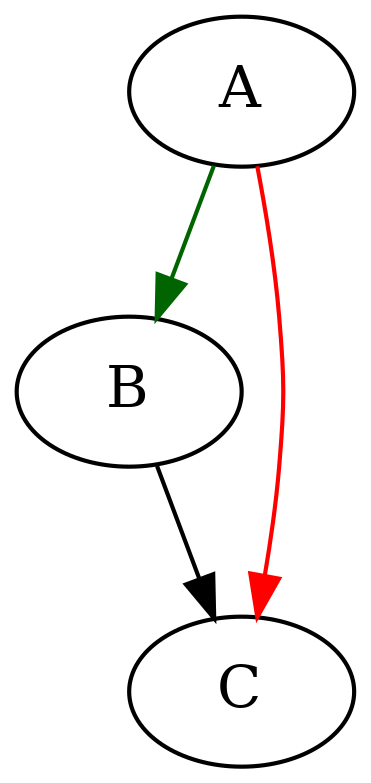
\includegraphics[width=0.4\textwidth]{inc/methods/hammock/if.png}
			\caption{Canonical 1-way conditional.}
		\end{subfigure}
		\quad
		\begin{subfigure}[b]{0.65\textwidth}
			\centering
			\begin{subfigure}[ht]{0.40\textwidth}
				\centering
				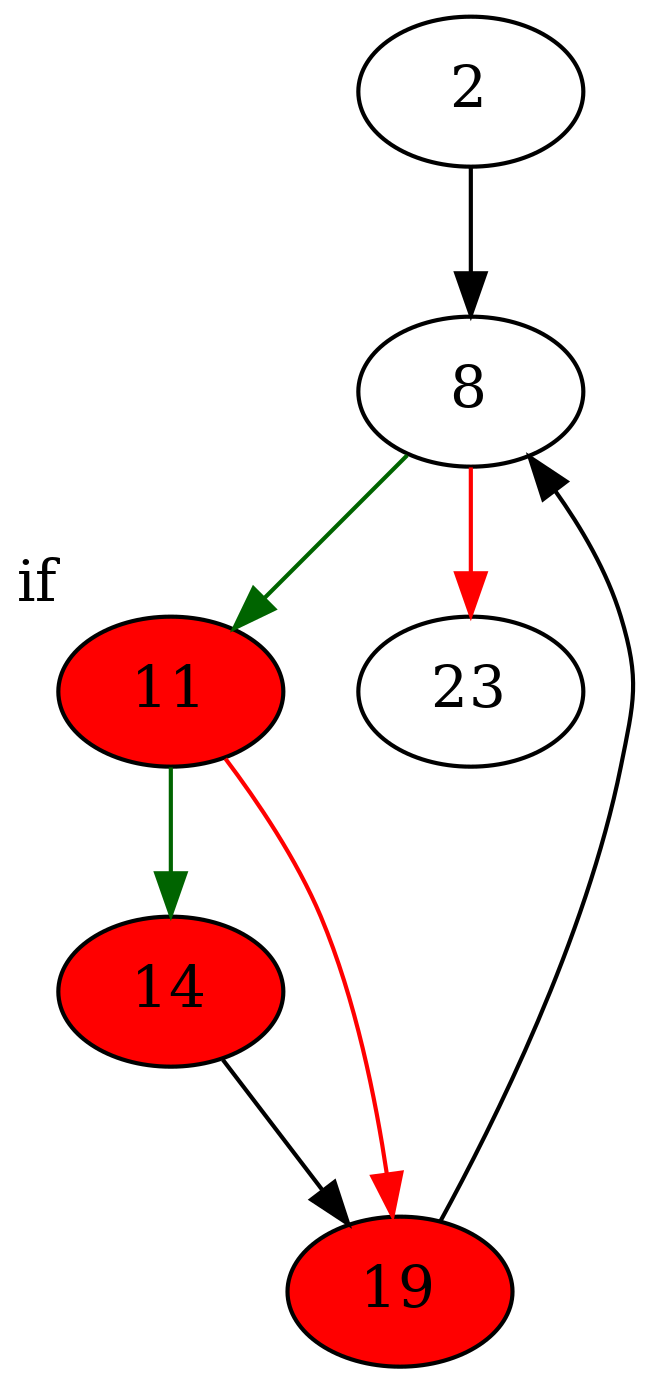
\includegraphics[width=0.5\textwidth]{inc/methods/hammock/main_0002a.png}
			\end{subfigure}
			\quad
			\begin{subfigure}[ht]{0.40\textwidth}
				\centering
				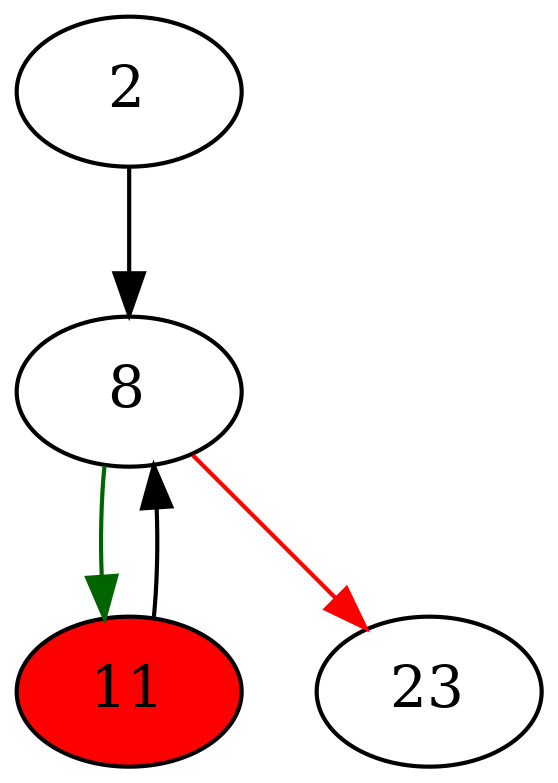
\includegraphics[width=0.5\textwidth]{inc/methods/hammock/main_0002b.png}
			\end{subfigure}
			\caption{Subgraph isomorphism of canonical 1-way conditional located in control flow graph (left) and its nodes merged (right).}
		\end{subfigure}
	\end{figure}
\end{frame}

% ___ [ Hammock - Example ] ____________________________________________________

% One example for each method, how it works.

\begin{frame}
	\frametitle{Hammock method - example}
	Example with nested control flow primitives.
	\begin{figure}[htbp]
		\centering
		\begin{subfigure}[b]{0.30\textwidth}
			\centering
			\lstinputlisting[language=C, style=c, basicstyle=\tiny\ttfamily, breaklines=false]{inc/methods/hammock/example/without-break.c}
			\caption{Original C source code.}
		\end{subfigure}
		\begin{subfigure}[b]{0.50\textwidth}
			\centering
			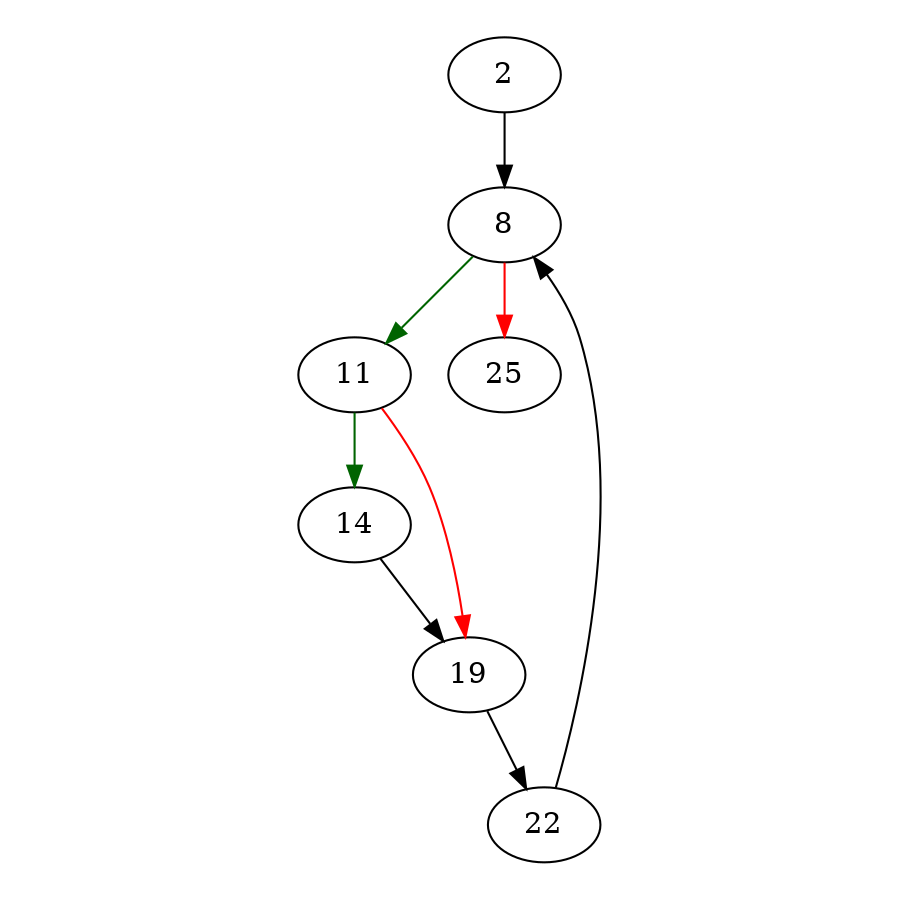
\includegraphics[height=0.6\paperheight]{inc/methods/hammock/example/without-break/main.png}
			\caption{Control flow graph.}
		\end{subfigure}
	\end{figure}
\end{frame}

\begin{frame}[noframenumbering]
	\frametitle{Hammock method - example}
	Example with nested control flow primitives.
	\begin{figure}[htbp]
		\centering
		\begin{subfigure}[b]{0.30\textwidth}
			\centering
			\lstinputlisting[linebackgroundcolor={\btLstHL{9-10}}, language=C, style=c, basicstyle=\tiny\ttfamily, breaklines=false]{inc/methods/hammock/example/without-break.c}
			\caption{Original C source code.}
		\end{subfigure}
		\begin{subfigure}[b]{0.50\textwidth}
			\centering
			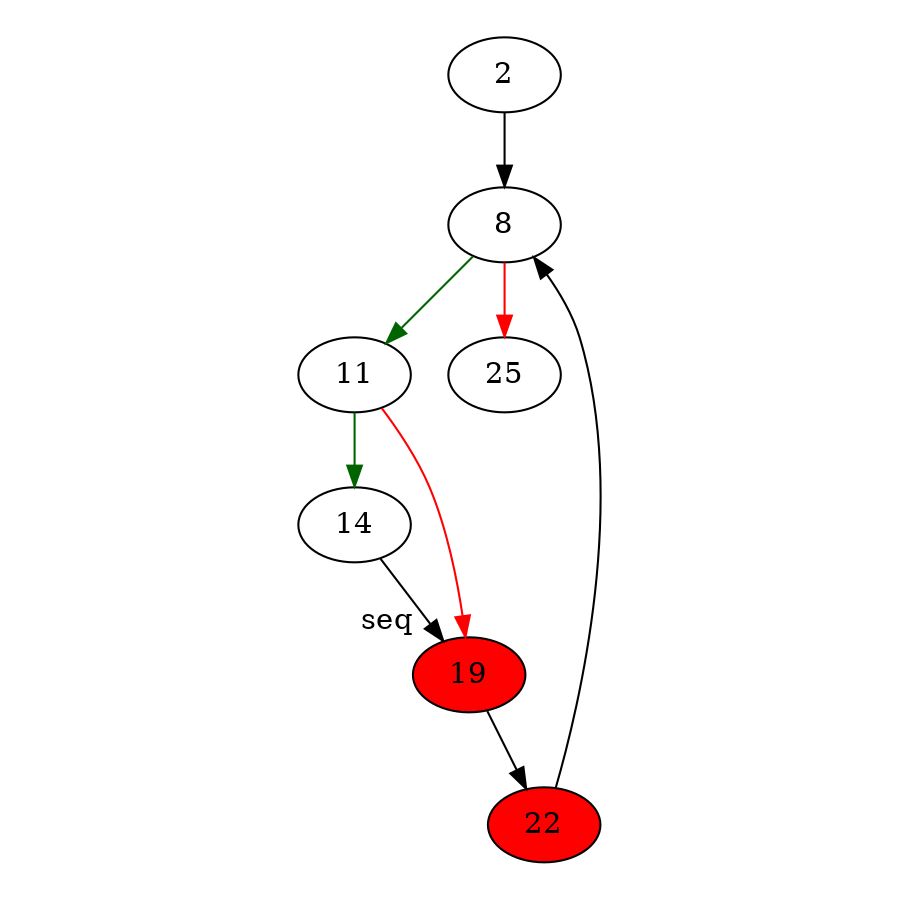
\includegraphics[height=0.6\paperheight]{inc/methods/hammock/example/without-break/main_0001a.png}
			\caption{Control flow graph.}
		\end{subfigure}
	\end{figure}
\end{frame}

\begin{frame}[noframenumbering]
	\frametitle{Hammock method - example}
	Example with nested control flow primitives.
	\begin{figure}[htbp]
		\centering
		\begin{subfigure}[b]{0.30\textwidth}
			\centering
			\lstinputlisting[linebackgroundcolor={\btLstHL{9-10}}, language=C, style=c, basicstyle=\tiny\ttfamily, breaklines=false]{inc/methods/hammock/example/without-break.c}
			\caption{Original C source code.}
		\end{subfigure}
		\begin{subfigure}[b]{0.50\textwidth}
			\centering
			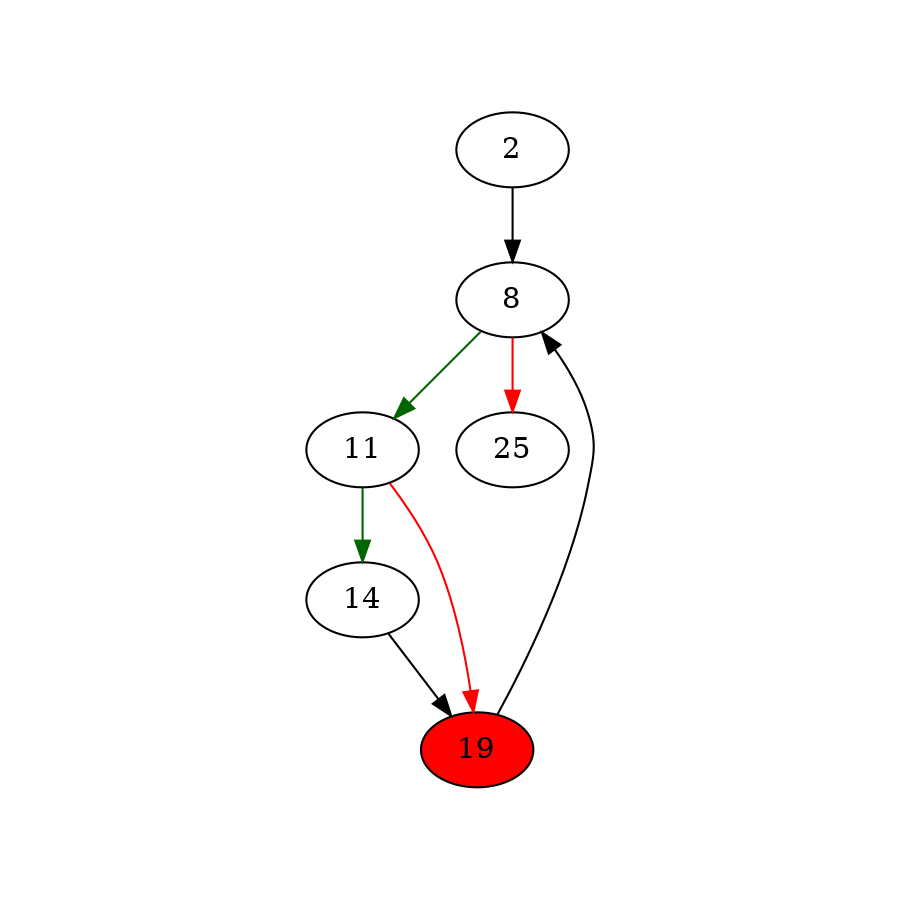
\includegraphics[height=0.6\paperheight]{inc/methods/hammock/example/without-break/main_0001b.png}
			\caption{Control flow graph.}
		\end{subfigure}
	\end{figure}
\end{frame}

\begin{frame}[noframenumbering]
	\frametitle{Hammock method - example}
	Example with nested control flow primitives.
	\begin{figure}[htbp]
		\centering
		\begin{subfigure}[b]{0.30\textwidth}
			\centering
			\lstinputlisting[linebackgroundcolor={\btLstHL{6-8}}, language=C, style=c, basicstyle=\tiny\ttfamily, breaklines=false]{inc/methods/hammock/example/without-break.c}
			\caption{Original C source code.}
		\end{subfigure}
		\begin{subfigure}[b]{0.50\textwidth}
			\centering
			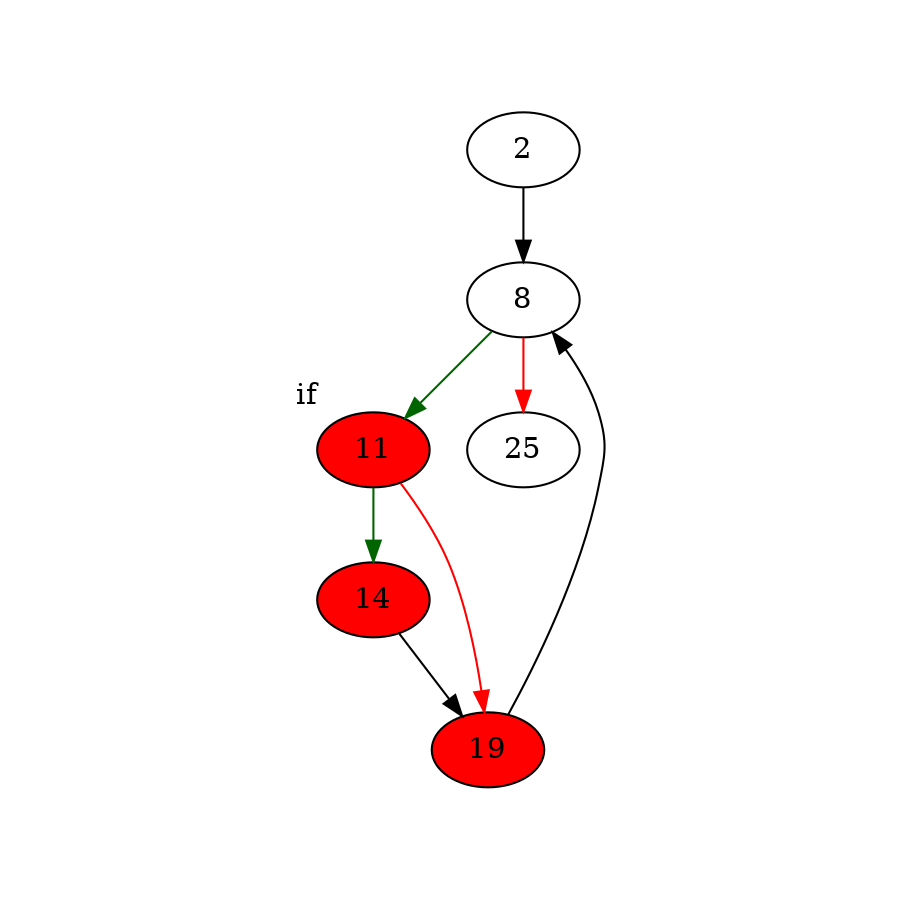
\includegraphics[height=0.6\paperheight]{inc/methods/hammock/example/without-break/main_0002a.png}
			\caption{Control flow graph.}
		\end{subfigure}
	\end{figure}
\end{frame}

\begin{frame}[noframenumbering]
	\frametitle{Hammock method - example}
	Example with nested control flow primitives.
	\begin{figure}[htbp]
		\centering
		\begin{subfigure}[b]{0.30\textwidth}
			\centering
			\lstinputlisting[linebackgroundcolor={\btLstHL{6-8}}, language=C, style=c, basicstyle=\tiny\ttfamily, breaklines=false]{inc/methods/hammock/example/without-break.c}
			\caption{Original C source code.}
		\end{subfigure}
		\begin{subfigure}[b]{0.50\textwidth}
			\centering
			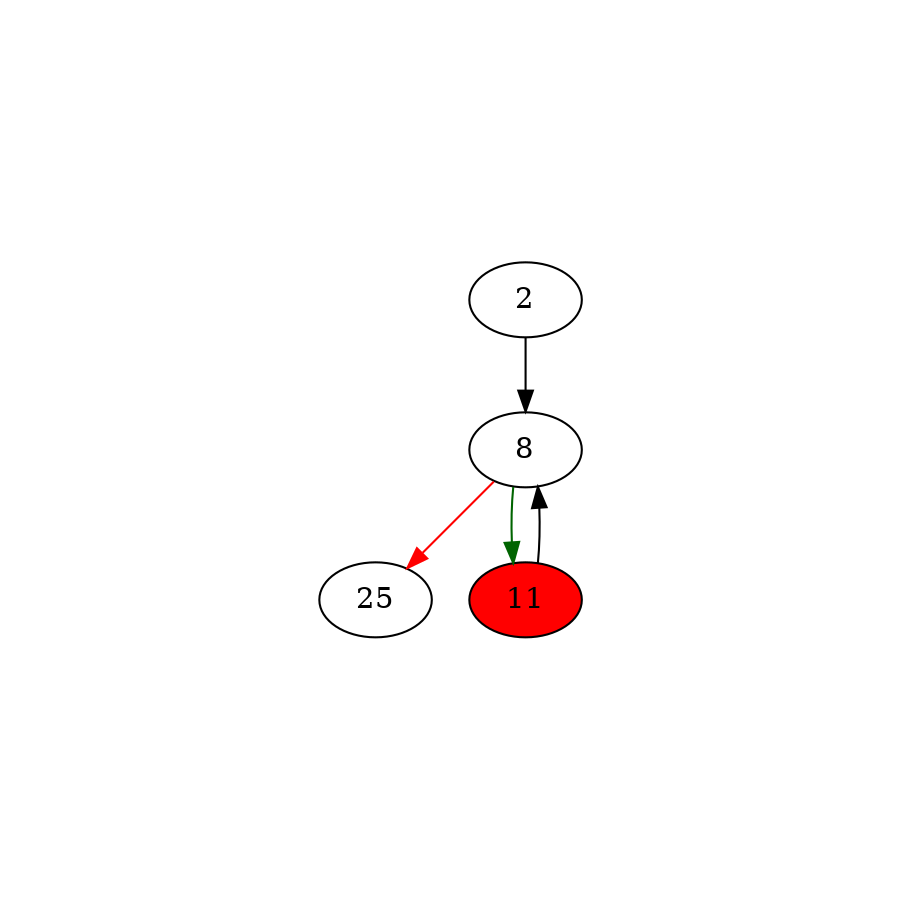
\includegraphics[height=0.6\paperheight]{inc/methods/hammock/example/without-break/main_0002b.png}
			\caption{Control flow graph.}
		\end{subfigure}
	\end{figure}
\end{frame}

\begin{frame}[noframenumbering]
	\frametitle{Hammock method - example}
	Example with nested control flow primitives.
	\begin{figure}[htbp]
		\centering
		\begin{subfigure}[b]{0.30\textwidth}
			\centering
			\lstinputlisting[linebackgroundcolor={\btLstHL{5, 10}}, language=C, style=c, basicstyle=\tiny\ttfamily, breaklines=false]{inc/methods/hammock/example/without-break.c}
			\caption{Original C source code.}
		\end{subfigure}
		\begin{subfigure}[b]{0.50\textwidth}
			\centering
			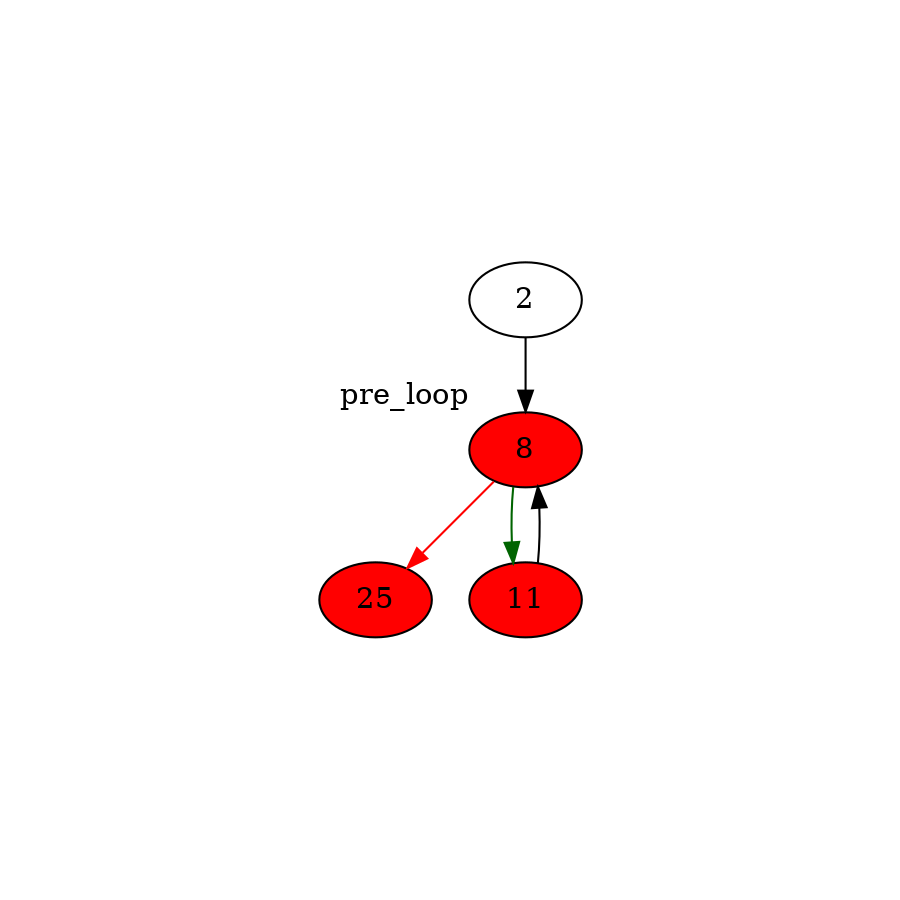
\includegraphics[height=0.6\paperheight]{inc/methods/hammock/example/without-break/main_0003a.png}
			\caption{Control flow graph.}
		\end{subfigure}
	\end{figure}
\end{frame}

\begin{frame}[noframenumbering]
	\frametitle{Hammock method - example}
	Example with nested control flow primitives.
	\begin{figure}[htbp]
		\centering
		\begin{subfigure}[b]{0.30\textwidth}
			\centering
			\lstinputlisting[linebackgroundcolor={\btLstHL{5, 10}}, language=C, style=c, basicstyle=\tiny\ttfamily, breaklines=false]{inc/methods/hammock/example/without-break.c}
			\caption{Original C source code.}
		\end{subfigure}
		\begin{subfigure}[b]{0.50\textwidth}
			\centering
			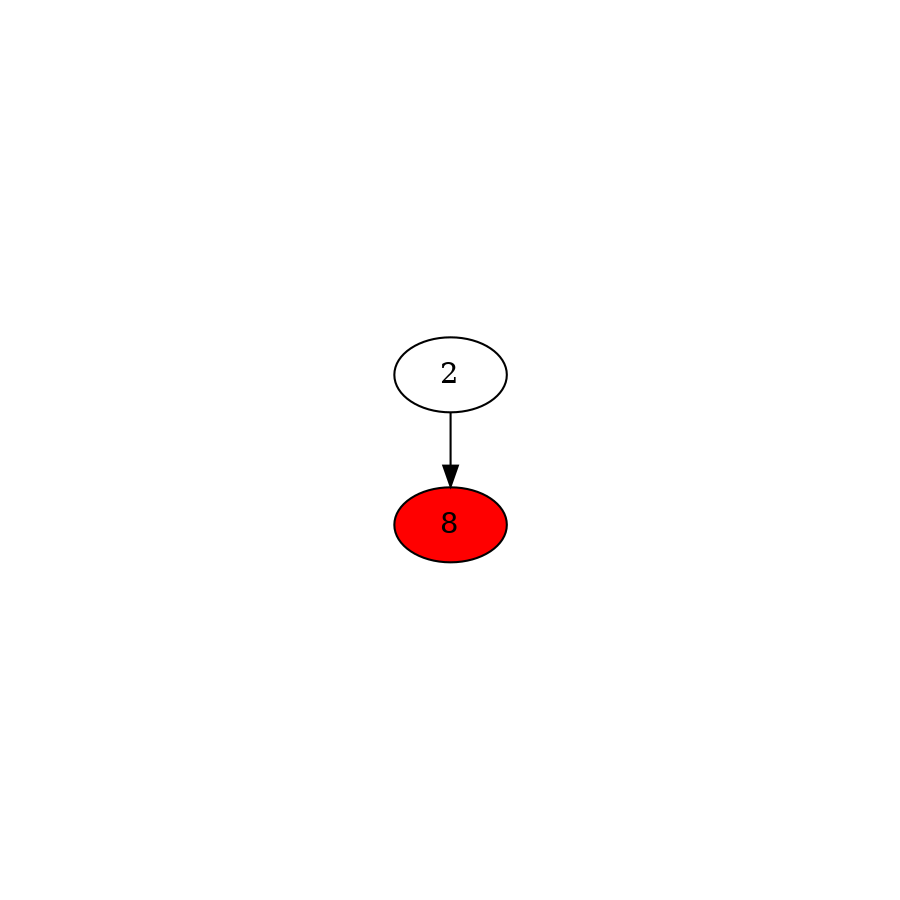
\includegraphics[height=0.6\paperheight]{inc/methods/hammock/example/without-break/main_0003b.png}
			\caption{Control flow graph.}
		\end{subfigure}
	\end{figure}
\end{frame}

\begin{frame}[noframenumbering]
	\frametitle{Hammock method - example}
	Example with nested control flow primitives.
	\begin{figure}[htbp]
		\centering
		\begin{subfigure}[b]{0.30\textwidth}
			\centering
			\lstinputlisting[linebackgroundcolor={\btLstHL{2-4}}, language=C, style=c, basicstyle=\tiny\ttfamily, breaklines=false]{inc/methods/hammock/example/without-break.c}
			\caption{Original C source code.}
		\end{subfigure}
		\begin{subfigure}[b]{0.50\textwidth}
			\centering
			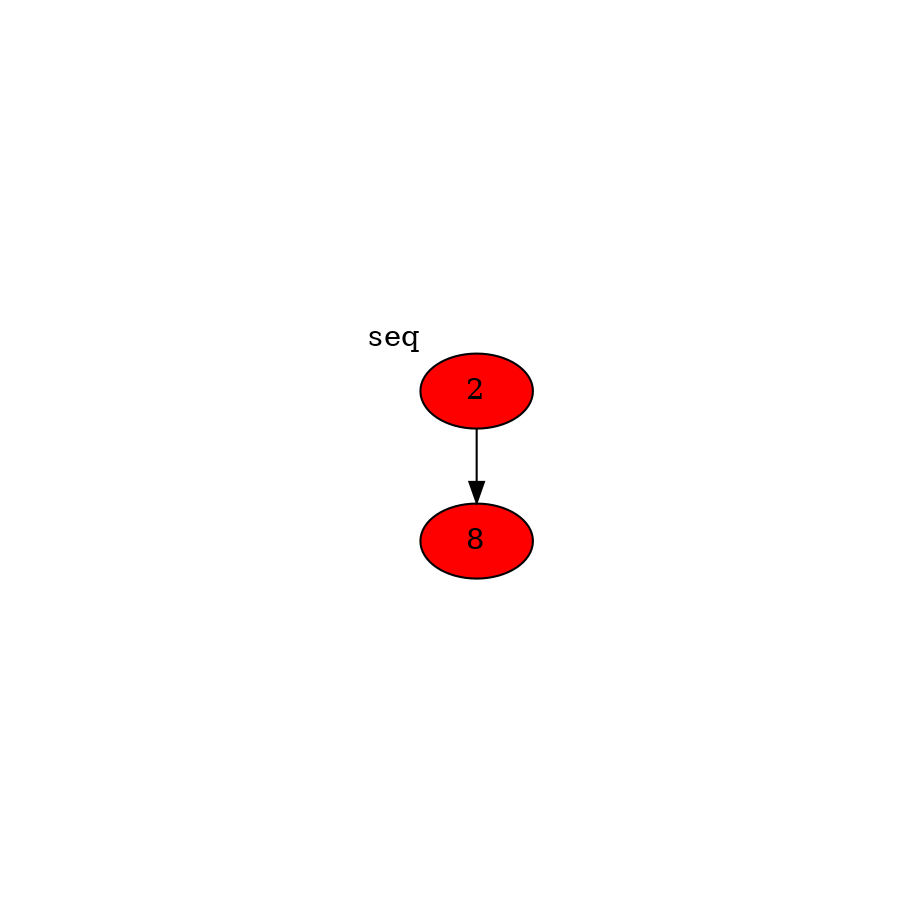
\includegraphics[height=0.6\paperheight]{inc/methods/hammock/example/without-break/main_0004a.png}
			\caption{Control flow graph.}
		\end{subfigure}
	\end{figure}
\end{frame}

\begin{frame}[noframenumbering]
	\frametitle{Hammock method - example}
	Example with nested control flow primitives.
	\begin{figure}[htbp]
		\centering
		\begin{subfigure}[b]{0.30\textwidth}
			\centering
			\lstinputlisting[linebackgroundcolor={\btLstHL{2-4}}, language=C, style=c, basicstyle=\tiny\ttfamily, breaklines=false]{inc/methods/hammock/example/without-break.c}
			\caption{Original C source code.}
		\end{subfigure}
		\begin{subfigure}[b]{0.50\textwidth}
			\centering
			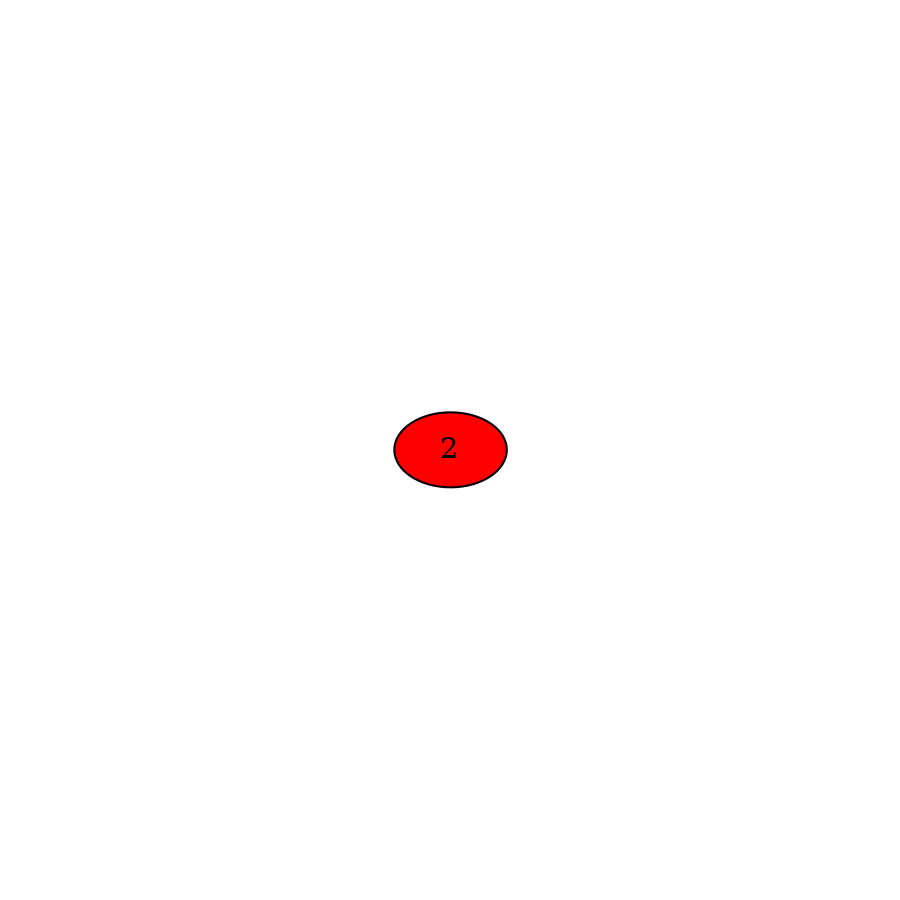
\includegraphics[height=0.6\paperheight]{inc/methods/hammock/example/without-break/main_0004b.png}
			\caption{Control flow graph; analysis \textbf{complete}.}
		\end{subfigure}
	\end{figure}
\end{frame}

% ___ [ Hammock - Counter-example 1 ] __________________________________________

% One example for each method, counter-example when it doesn't work.

% Multi-exit loops.

\begin{frame}
	\frametitle{Hammock method - counter-example 1}
	Counter-example with \textit{multi-exit loop}.
	\begin{figure}[htbp]
		\centering
		\begin{subfigure}[b]{0.30\textwidth}
			\centering
			\lstinputlisting[language=C, style=c, basicstyle=\tiny\ttfamily, breaklines=false]{inc/methods/hammock/counter-example/with-break.c}
			\caption{Original C source code.}
		\end{subfigure}
		\begin{subfigure}[b]{0.50\textwidth}
			\centering
			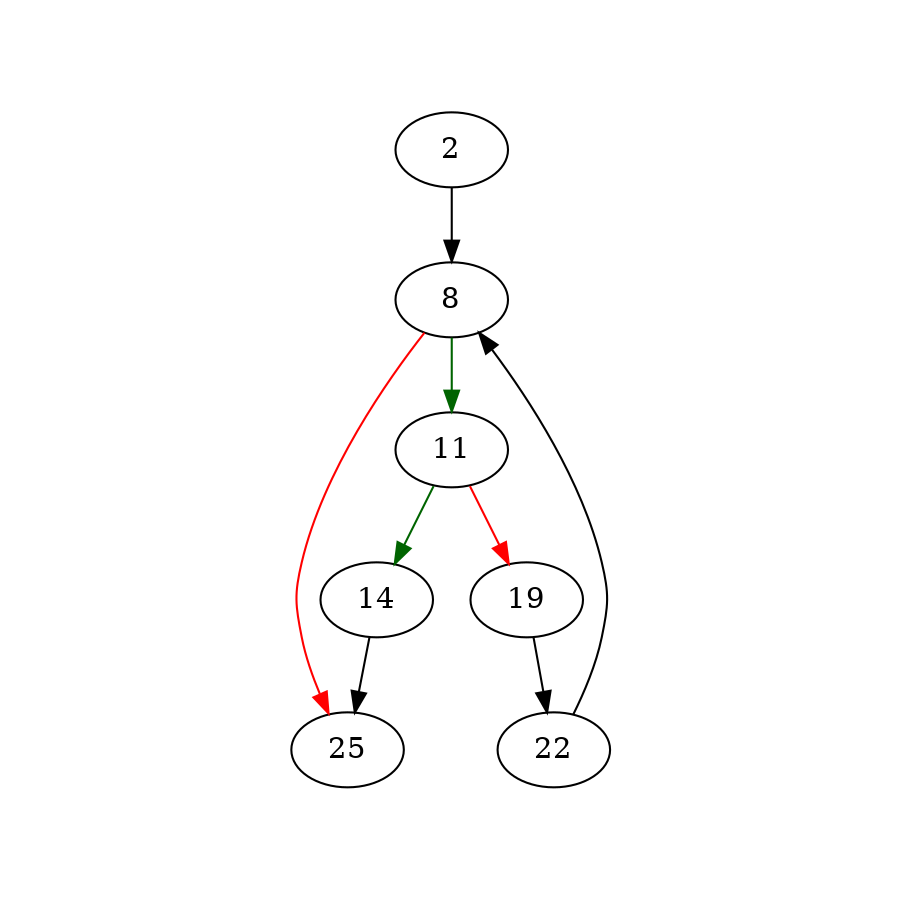
\includegraphics[height=0.6\paperheight]{inc/methods/hammock/counter-example/with-break/main.png}
			\caption{Control flow graph.}
		\end{subfigure}
	\end{figure}
\end{frame}

\begin{frame}[noframenumbering]
	\frametitle{Hammock method - counter-example 1}
	Counter-example with \textit{multi-exit loop}.
	\begin{figure}[htbp]
		\centering
		\begin{subfigure}[b]{0.30\textwidth}
			\centering
			\lstinputlisting[linebackgroundcolor={\btLstHL{10-11}}, language=C, style=c, basicstyle=\tiny\ttfamily, breaklines=false]{inc/methods/hammock/counter-example/with-break.c}
			\caption{Original C source code.}
		\end{subfigure}
		\begin{subfigure}[b]{0.50\textwidth}
			\centering
			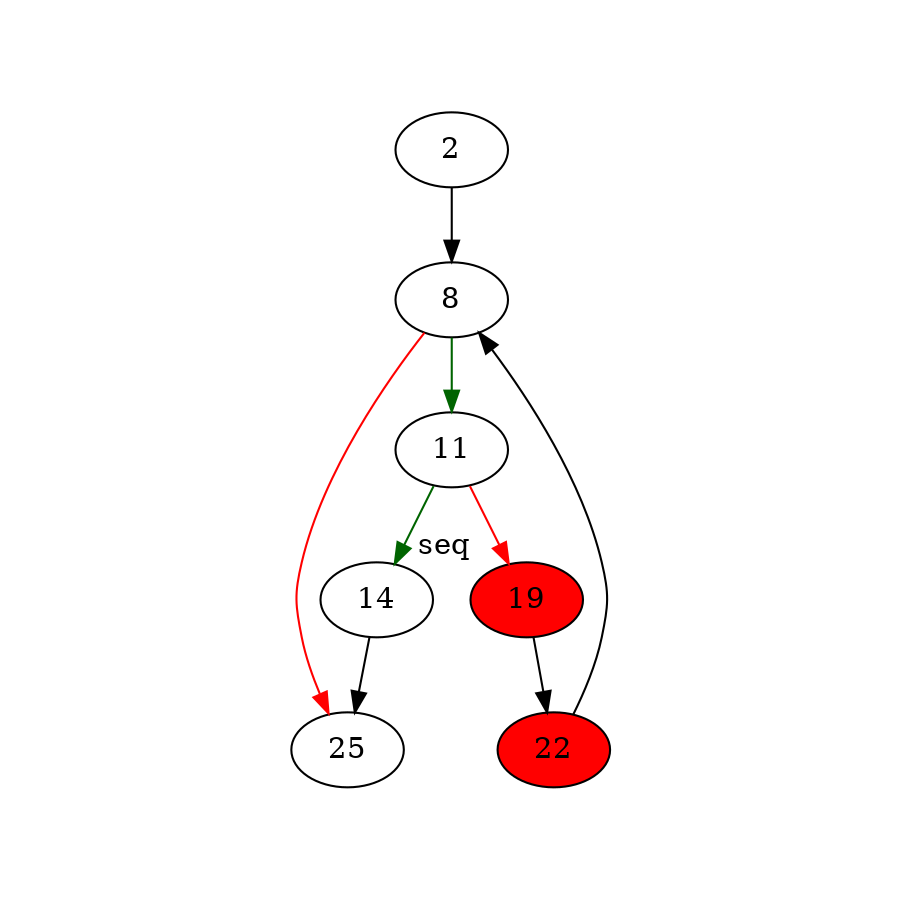
\includegraphics[height=0.6\paperheight]{inc/methods/hammock/counter-example/with-break/main_0001a.png}
			\caption{Control flow graph.}
		\end{subfigure}
	\end{figure}
\end{frame}

\begin{frame}[noframenumbering]
	\frametitle{Hammock method - counter-example 1}
	Counter-example with \textit{multi-exit loop}.
	\begin{figure}[htbp]
		\centering
		\begin{subfigure}[b]{0.30\textwidth}
			\centering
			\lstinputlisting[linebackgroundcolor={\btLstHL{10-11}}, language=C, style=c, basicstyle=\tiny\ttfamily, breaklines=false]{inc/methods/hammock/counter-example/with-break.c}
			\caption{Original C source code.}
		\end{subfigure}
		\begin{subfigure}[b]{0.50\textwidth}
			\centering
			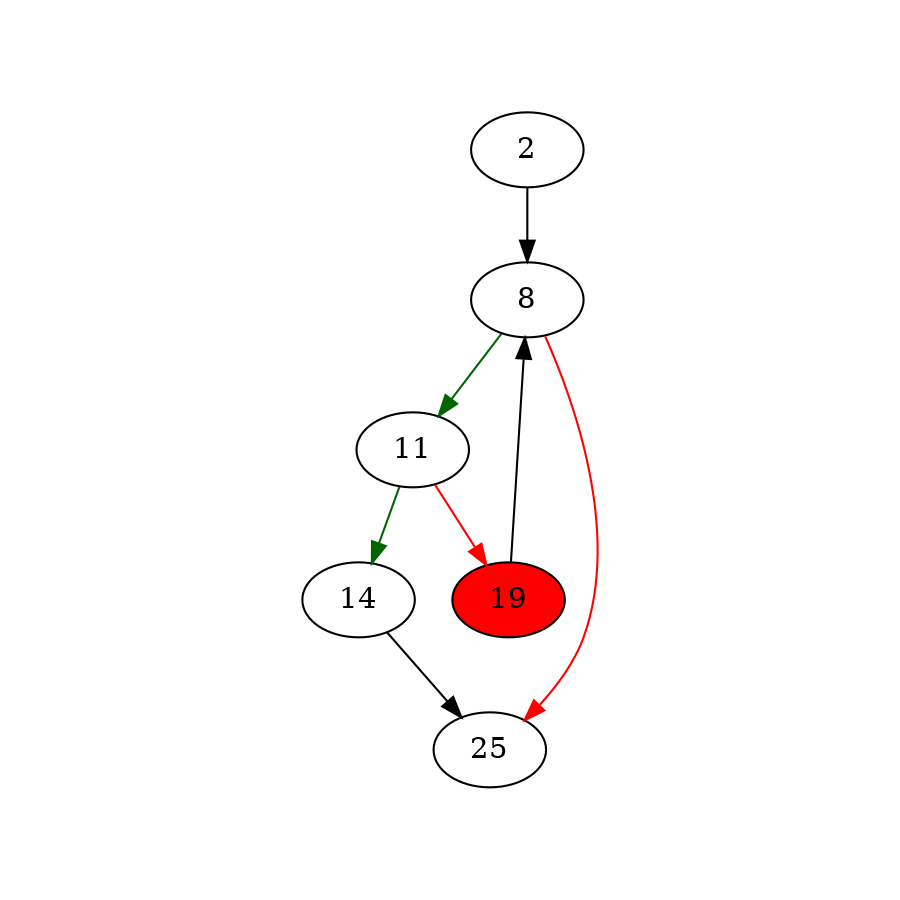
\includegraphics[height=0.6\paperheight]{inc/methods/hammock/counter-example/with-break/main_0001b.png}
			\caption{Control flow graph; analysis \textbf{incomplete}.}
		\end{subfigure}
	\end{figure}
\end{frame}

% ___ [ Hammock - Counter-example 2 ] __________________________________________

% One example for each method, counter-example when it doesn't work.

% Jump threading optimization and short-circuit evaluation.

\begin{frame}
	\frametitle{Hammock method - counter-example 2}
	Counter-example with \textit{jump threading} optimization and \textit{short-circuit} evaluation.
	\begin{figure}[htbp]
		\centering
		\begin{subfigure}[b]{0.30\textwidth}
			\centering
			\lstinputlisting[linerange={17-43}, language=C, style=c, basicstyle=\tiny\ttfamily, breaklines=false]{inc/methods/hammock/counter-example/jump-threading-and-short-circuit/jump-threading-and-short-circuit.c}
			\caption{Original C source code.}
		\end{subfigure}
		\begin{subfigure}[b]{0.50\textwidth}
			\centering
			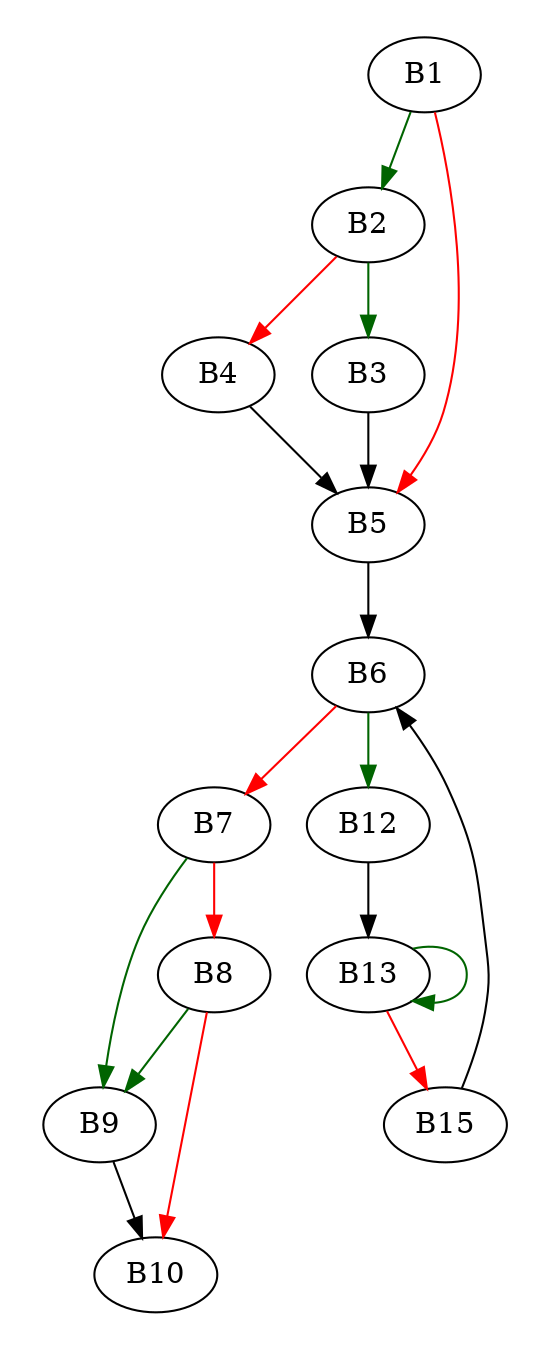
\includegraphics[height=0.7\paperheight]{inc/methods/hammock/counter-example/jump-threading-and-short-circuit/jump-threading-and-short-circuit_jump/f.png}
			\caption{Control flow graph.}
		\end{subfigure}
	\end{figure}
\end{frame}

\begin{frame}[noframenumbering]
	\frametitle{Hammock method - counter-example 2}
	Counter-example with \textit{jump threading} optimization and \textit{short-circuit} evaluation.
	\begin{figure}[htbp]
		\centering
		\begin{subfigure}[b]{0.30\textwidth}
			\centering
			\lstinputlisting[linebackgroundcolor={\btLstHL{15-18}}, linerange={17-43}, language=C, style=c, basicstyle=\tiny\ttfamily, breaklines=false]{inc/methods/hammock/counter-example/jump-threading-and-short-circuit/jump-threading-and-short-circuit.c}
			\caption{Original C source code.}
		\end{subfigure}
		\begin{subfigure}[b]{0.50\textwidth}
			\centering
			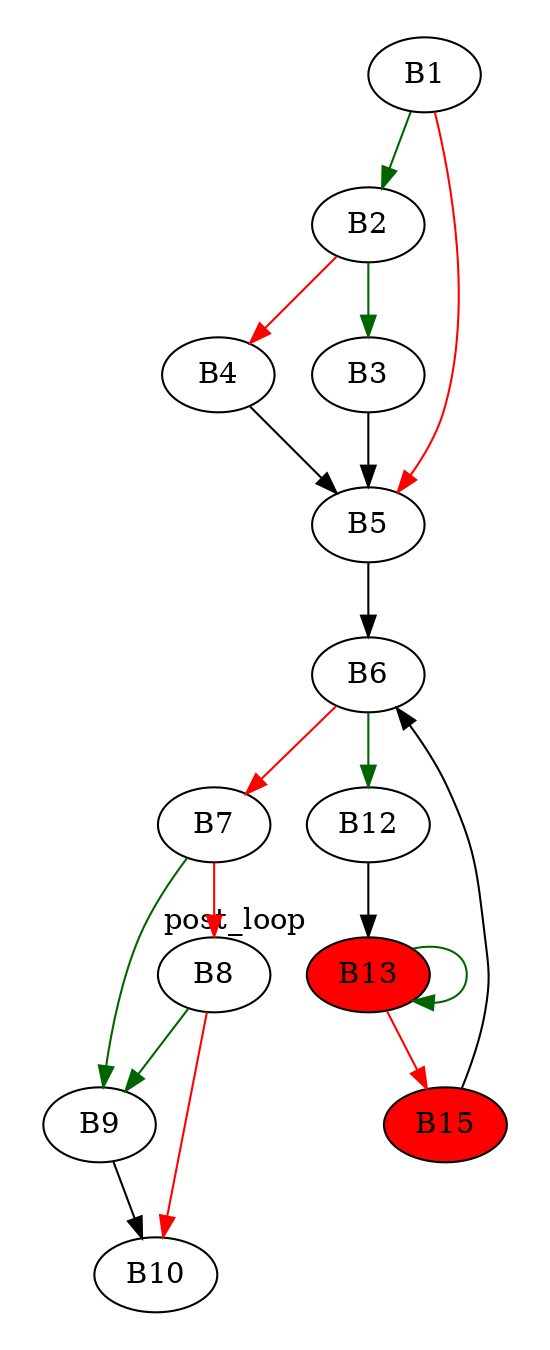
\includegraphics[height=0.7\paperheight]{inc/methods/hammock/counter-example/jump-threading-and-short-circuit/jump-threading-and-short-circuit_jump/f_0001a.png}
			\caption{Control flow graph.}
		\end{subfigure}
	\end{figure}
\end{frame}

\begin{frame}[noframenumbering]
	\frametitle{Hammock method - counter-example 2}
	Counter-example with \textit{jump threading} optimization and \textit{short-circuit} evaluation.
	\begin{figure}[htbp]
		\centering
		\begin{subfigure}[b]{0.30\textwidth}
			\centering
			\lstinputlisting[linebackgroundcolor={\btLstHL{15-18}}, linerange={17-43}, language=C, style=c, basicstyle=\tiny\ttfamily, breaklines=false]{inc/methods/hammock/counter-example/jump-threading-and-short-circuit/jump-threading-and-short-circuit.c}
			\caption{Original C source code.}
		\end{subfigure}
		\begin{subfigure}[b]{0.50\textwidth}
			\centering
			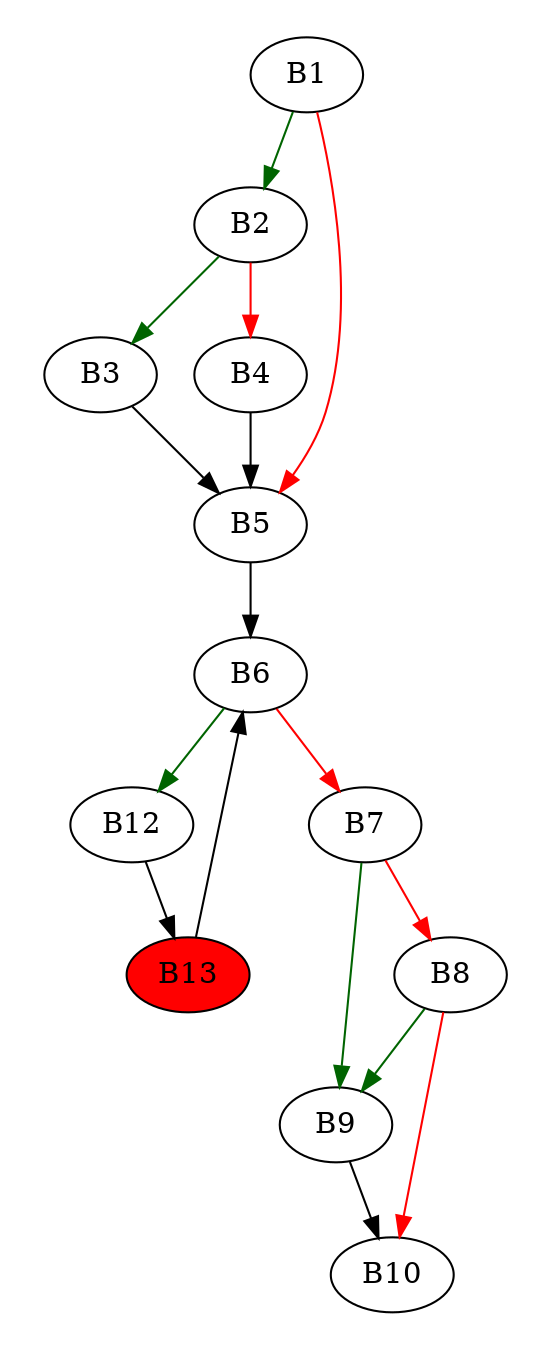
\includegraphics[height=0.7\paperheight]{inc/methods/hammock/counter-example/jump-threading-and-short-circuit/jump-threading-and-short-circuit_jump/f_0001b.png}
			\caption{Control flow graph.}
		\end{subfigure}
	\end{figure}
\end{frame}

\begin{frame}[noframenumbering]
	\frametitle{Hammock method - counter-example 2}
	Counter-example with \textit{jump threading} optimization and \textit{short-circuit} evaluation.
	\begin{figure}[htbp]
		\centering
		\begin{subfigure}[b]{0.30\textwidth}
			\centering
			\lstinputlisting[linebackgroundcolor={\btLstHL{13-14}}, linerange={17-43}, language=C, style=c, basicstyle=\tiny\ttfamily, breaklines=false]{inc/methods/hammock/counter-example/jump-threading-and-short-circuit/jump-threading-and-short-circuit.c}
			\caption{Original C source code.}
		\end{subfigure}
		\begin{subfigure}[b]{0.50\textwidth}
			\centering
			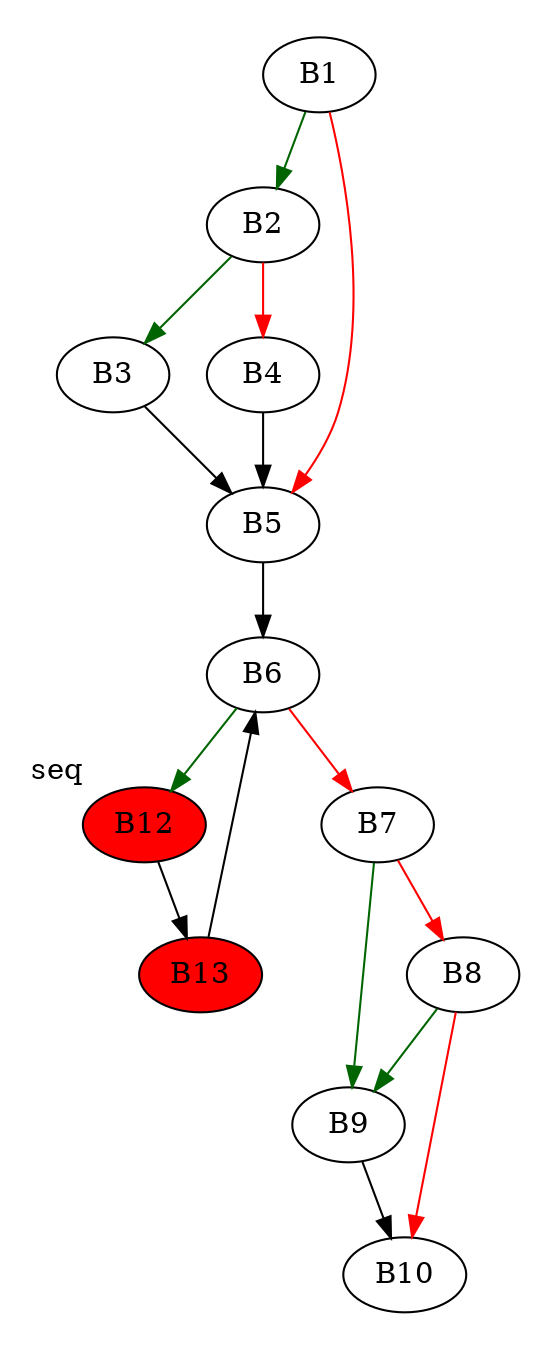
\includegraphics[height=0.7\paperheight]{inc/methods/hammock/counter-example/jump-threading-and-short-circuit/jump-threading-and-short-circuit_jump/f_0002a.png}
			\caption{Control flow graph.}
		\end{subfigure}
	\end{figure}
\end{frame}

\begin{frame}[noframenumbering]
	\frametitle{Hammock method - counter-example 2}
	Counter-example with \textit{jump threading} optimization and \textit{short-circuit} evaluation.
	\begin{figure}[htbp]
		\centering
		\begin{subfigure}[b]{0.30\textwidth}
			\centering
			\lstinputlisting[linebackgroundcolor={\btLstHL{13-14}}, linerange={17-43}, language=C, style=c, basicstyle=\tiny\ttfamily, breaklines=false]{inc/methods/hammock/counter-example/jump-threading-and-short-circuit/jump-threading-and-short-circuit.c}
			\caption{Original C source code.}
		\end{subfigure}
		\begin{subfigure}[b]{0.50\textwidth}
			\centering
			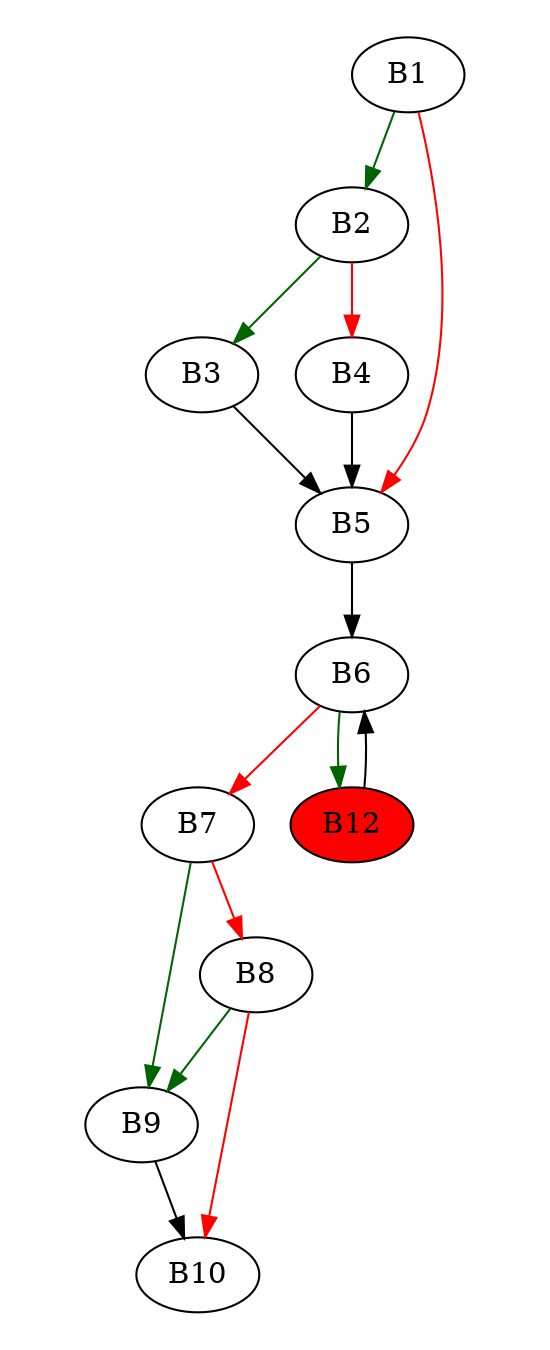
\includegraphics[height=0.7\paperheight]{inc/methods/hammock/counter-example/jump-threading-and-short-circuit/jump-threading-and-short-circuit_jump/f_0002b.png}
			\caption{Control flow graph.}
		\end{subfigure}
	\end{figure}
\end{frame}

\begin{frame}[noframenumbering]
	\frametitle{Hammock method - counter-example 2}
	Counter-example with \textit{jump threading} optimization and \textit{short-circuit} evaluation.
	\begin{figure}[htbp]
		\centering
		\begin{subfigure}[b]{0.30\textwidth}
			\centering
			\lstinputlisting[linebackgroundcolor={\btLstHL{12-13}}, linerange={17-43}, language=C, style=c, basicstyle=\tiny\ttfamily, breaklines=false]{inc/methods/hammock/counter-example/jump-threading-and-short-circuit/jump-threading-and-short-circuit.c}
			\caption{Original C source code.}
		\end{subfigure}
		\begin{subfigure}[b]{0.50\textwidth}
			\centering
			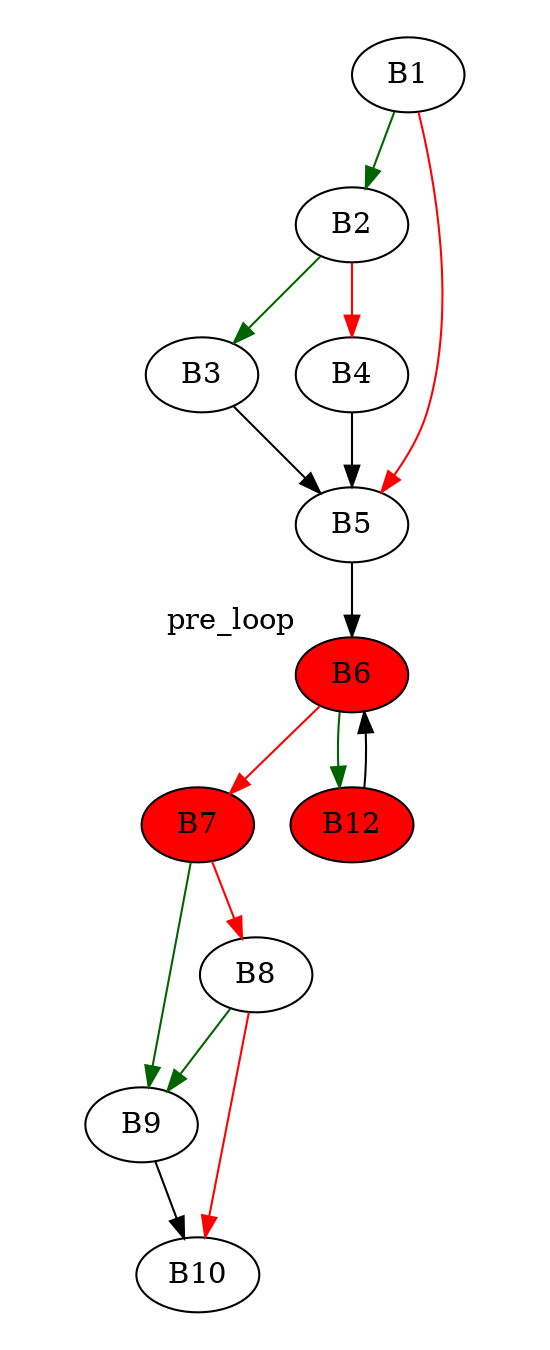
\includegraphics[height=0.7\paperheight]{inc/methods/hammock/counter-example/jump-threading-and-short-circuit/jump-threading-and-short-circuit_jump/f_0003a.png}
			\caption{Control flow graph.}
		\end{subfigure}
	\end{figure}
\end{frame}

\begin{frame}[noframenumbering]
	\frametitle{Hammock method - counter-example 2}
	Counter-example with \textit{jump threading} optimization and \textit{short-circuit} evaluation.
	\begin{figure}[htbp]
		\centering
		\begin{subfigure}[b]{0.30\textwidth}
			\centering
			\lstinputlisting[linebackgroundcolor={\btLstHL{12-13}}, linerange={17-43}, language=C, style=c, basicstyle=\tiny\ttfamily, breaklines=false]{inc/methods/hammock/counter-example/jump-threading-and-short-circuit/jump-threading-and-short-circuit.c}
			\caption{Original C source code.}
		\end{subfigure}
		\begin{subfigure}[b]{0.50\textwidth}
			\centering
			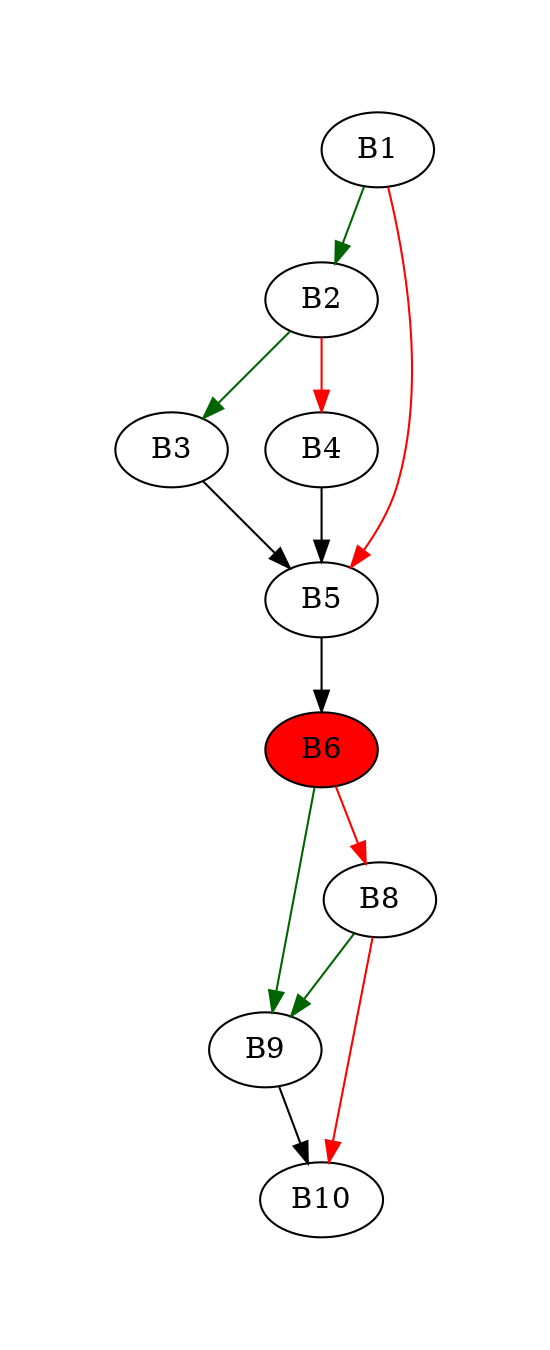
\includegraphics[height=0.7\paperheight]{inc/methods/hammock/counter-example/jump-threading-and-short-circuit/jump-threading-and-short-circuit_jump/f_0003b.png}
			\caption{Control flow graph.}
		\end{subfigure}
	\end{figure}
\end{frame}

\begin{frame}[noframenumbering]
	\frametitle{Hammock method - counter-example 2}
	Counter-example with \textit{jump threading} optimization and \textit{short-circuit} evaluation.
	\begin{figure}[htbp]
		\centering
		\begin{subfigure}[b]{0.30\textwidth}
			\centering
			\lstinputlisting[linebackgroundcolor={\btLstHL{11-12}}, linerange={17-43}, language=C, style=c, basicstyle=\tiny\ttfamily, breaklines=false]{inc/methods/hammock/counter-example/jump-threading-and-short-circuit/jump-threading-and-short-circuit.c}
			\caption{Original C source code.}
		\end{subfigure}
		\begin{subfigure}[b]{0.50\textwidth}
			\centering
			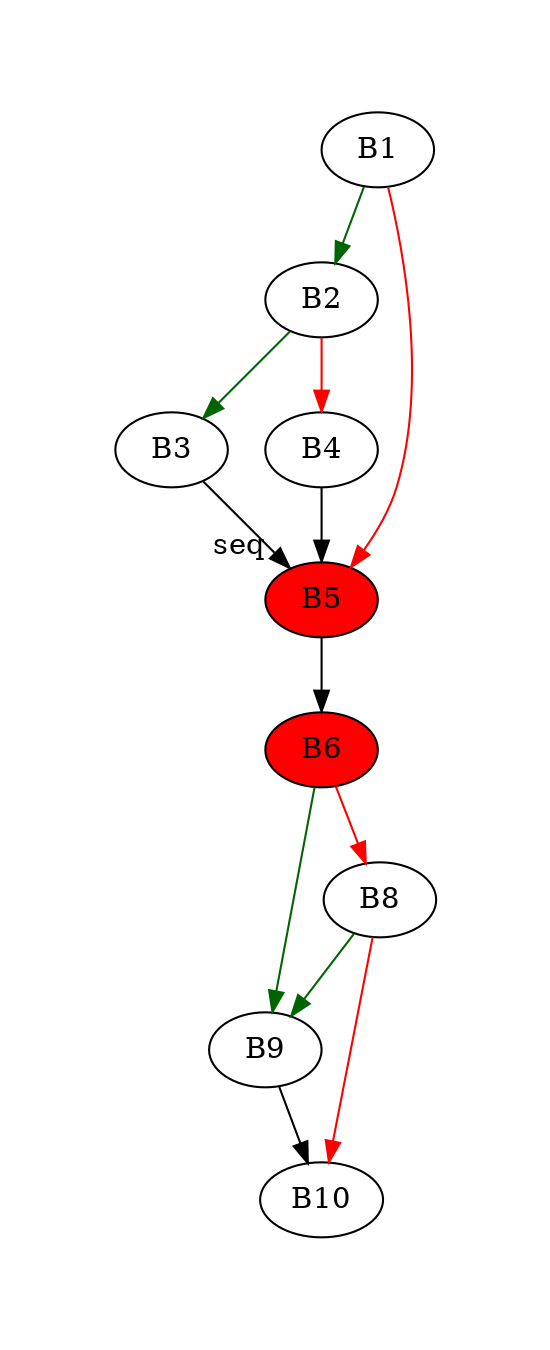
\includegraphics[height=0.7\paperheight]{inc/methods/hammock/counter-example/jump-threading-and-short-circuit/jump-threading-and-short-circuit_jump/f_0004a.png}
			\caption{Control flow graph.}
		\end{subfigure}
	\end{figure}
\end{frame}

\begin{frame}[noframenumbering]
	\frametitle{Hammock method - counter-example 2}
	Counter-example with \textit{jump threading} optimization and \textit{short-circuit} evaluation.
	\begin{figure}[htbp]
		\centering
		\begin{subfigure}[b]{0.30\textwidth}
			\centering
			\lstinputlisting[linebackgroundcolor={\btLstHL{11-12}}, linerange={17-43}, language=C, style=c, basicstyle=\tiny\ttfamily, breaklines=false]{inc/methods/hammock/counter-example/jump-threading-and-short-circuit/jump-threading-and-short-circuit.c}
			\caption{Original C source code.}
		\end{subfigure}
		\begin{subfigure}[b]{0.50\textwidth}
			\centering
			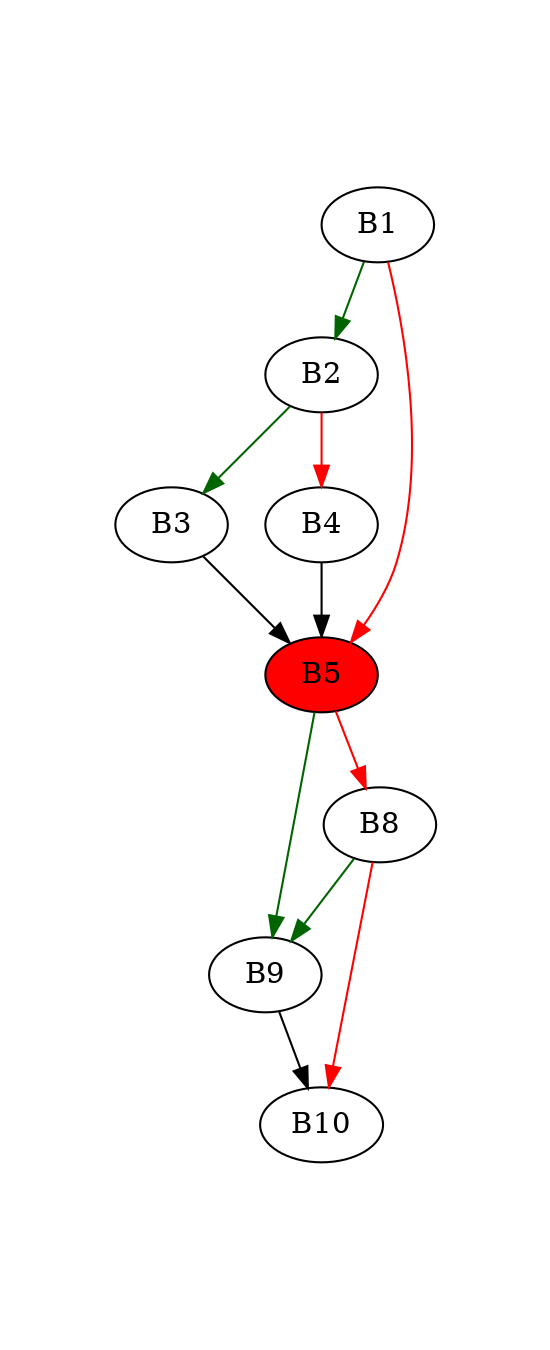
\includegraphics[height=0.7\paperheight]{inc/methods/hammock/counter-example/jump-threading-and-short-circuit/jump-threading-and-short-circuit_jump/f_0004b.png}
			\caption{Control flow graph; analysis \textbf{incomplete}.}
		\end{subfigure}
	\end{figure}
\end{frame}

% --- [ Interval method ] ------------------------------------------------------

\begin{frame}
	\frametitle{Interval method}

	Identify intervals in CFGs to determine the nesting-levels of loops and the follow nodes of high-level control flow primitives.

	\vspace*{2em}

	\begin{block}{Pros}
		\begin{itemize}
			\item handles multi-level \texttt{continue}- and \texttt{break}-statements in loops
			\item handles jump threading optimized control flow graphs
			\item handles short-circuit evaluation
		\end{itemize}
	\end{block}

	\begin{block}{Pros/Cons}
		\begin{itemize}
			\item \textit{some} false positives
			\item \textit{some} false negatives
		\end{itemize}
	\end{block}

\end{frame}

\begin{frame}
	\frametitle{Interval method}
	\begin{figure}[htbp]
		\begin{subfigure}[ht]{0.50\textwidth}
			\begin{subfigure}{\textwidth}
				Intervals have interesting properties.
			\end{subfigure}
			\vspace*{3em} \\
			\begin{subfigure}{\textwidth}
				\begin{quote}
					An \textbf{interval} $I(h)$ with header node $h$ is the maximal single-entry subgraph of a CFG in which $h$ is the only entry node and in which all cycles contain $h$.
				\end{quote}
			\end{subfigure}
		\end{subfigure}
		\begin{subfigure}[ht]{0.40\textwidth}
			\centering
			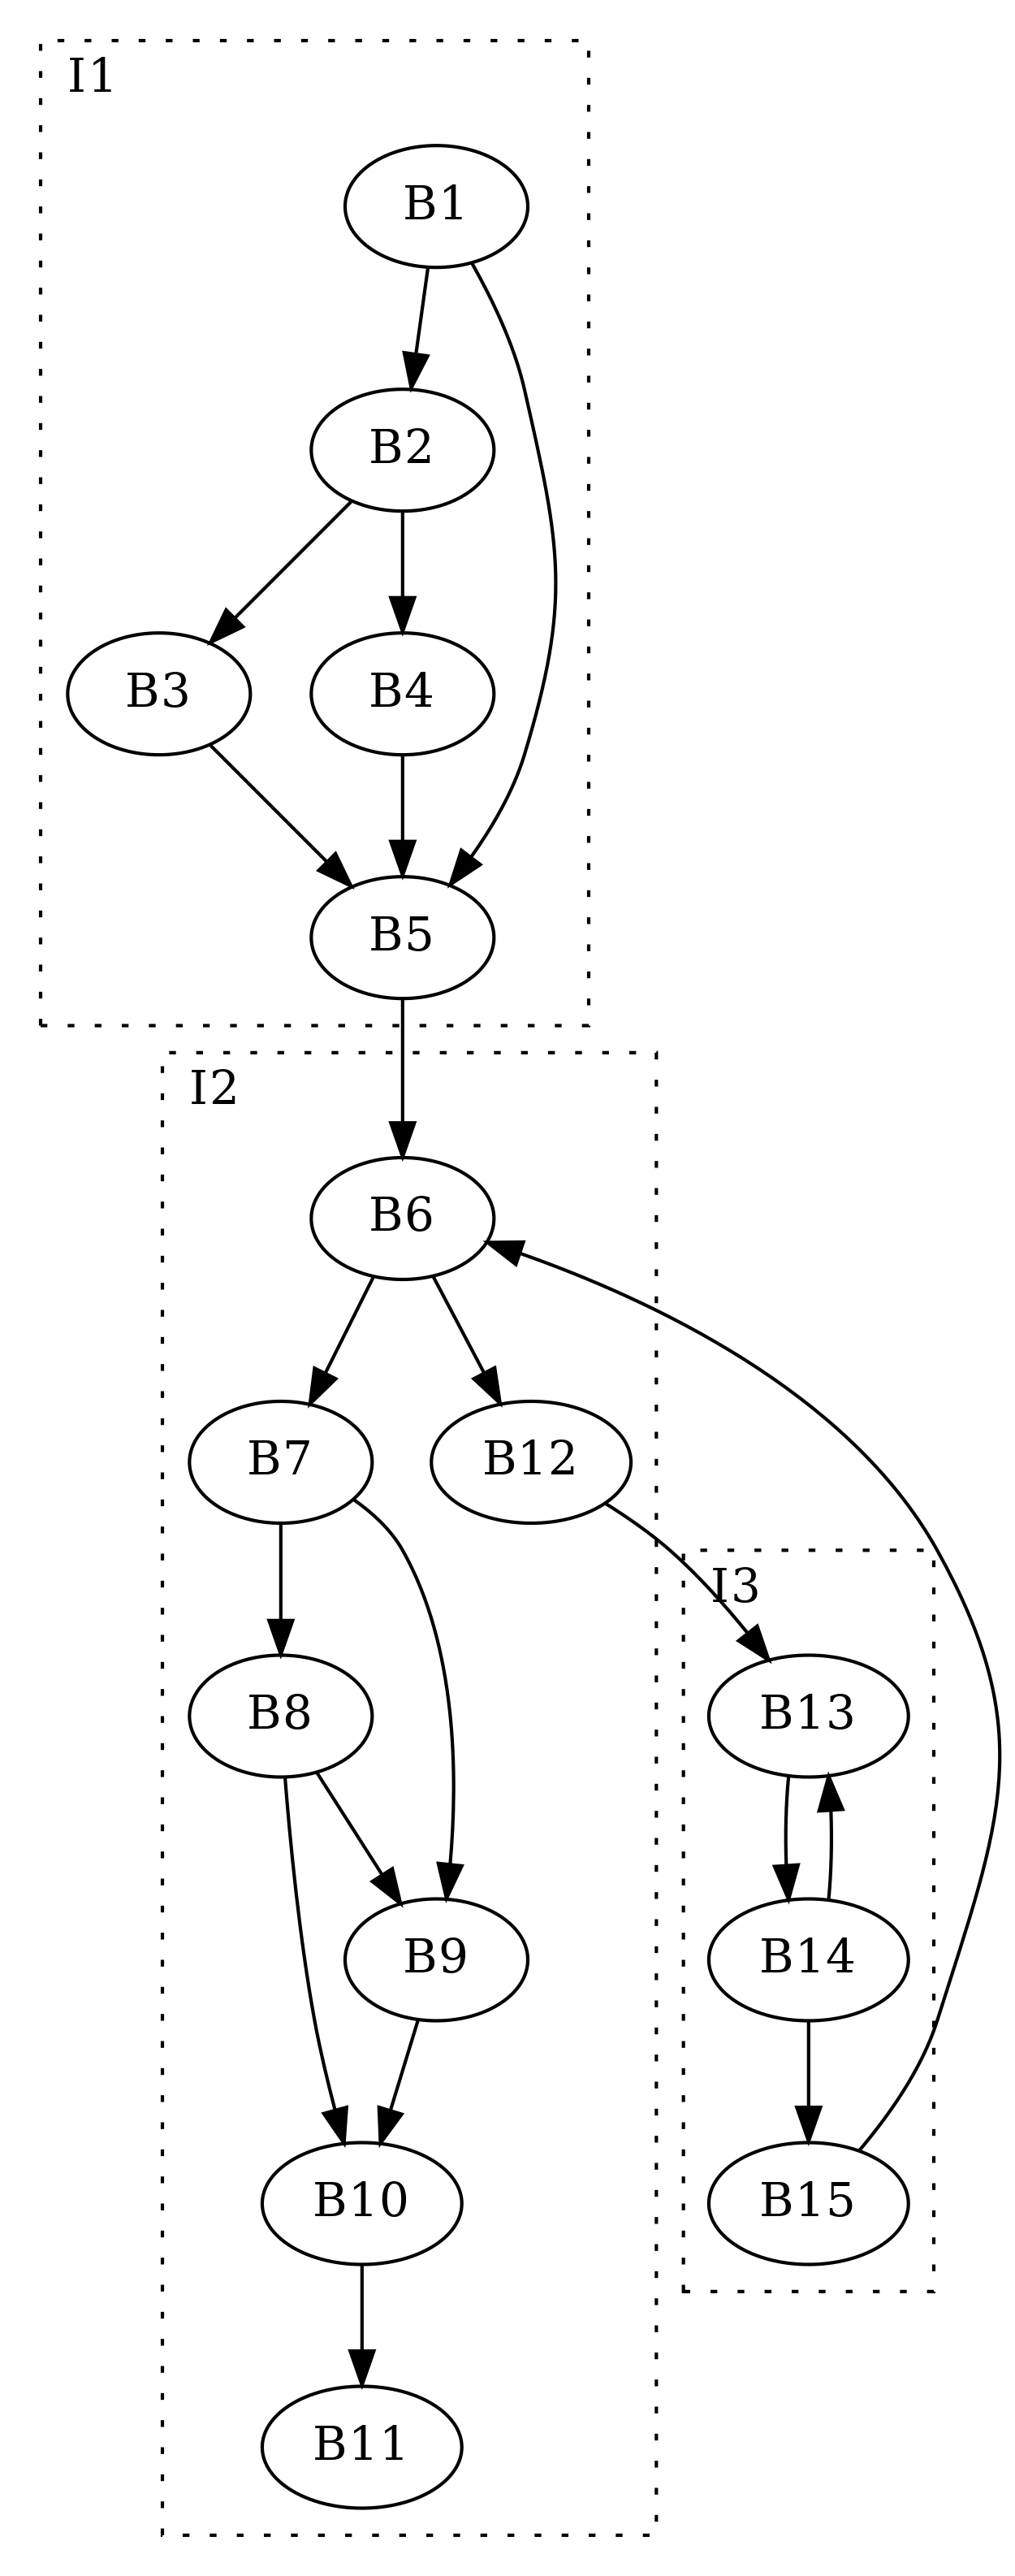
\includegraphics[height=0.75\textheight]{inc/methods/interval/G_1.png}
			\caption{Intervals outlined in control flow graph.}
		\end{subfigure}
	\end{figure}
\end{frame}

\begin{frame}
	\frametitle{Interval method}
	\begin{figure}[htbp]
		\centering
		\begin{subfigure}[b]{0.18\textwidth}
			\centering
			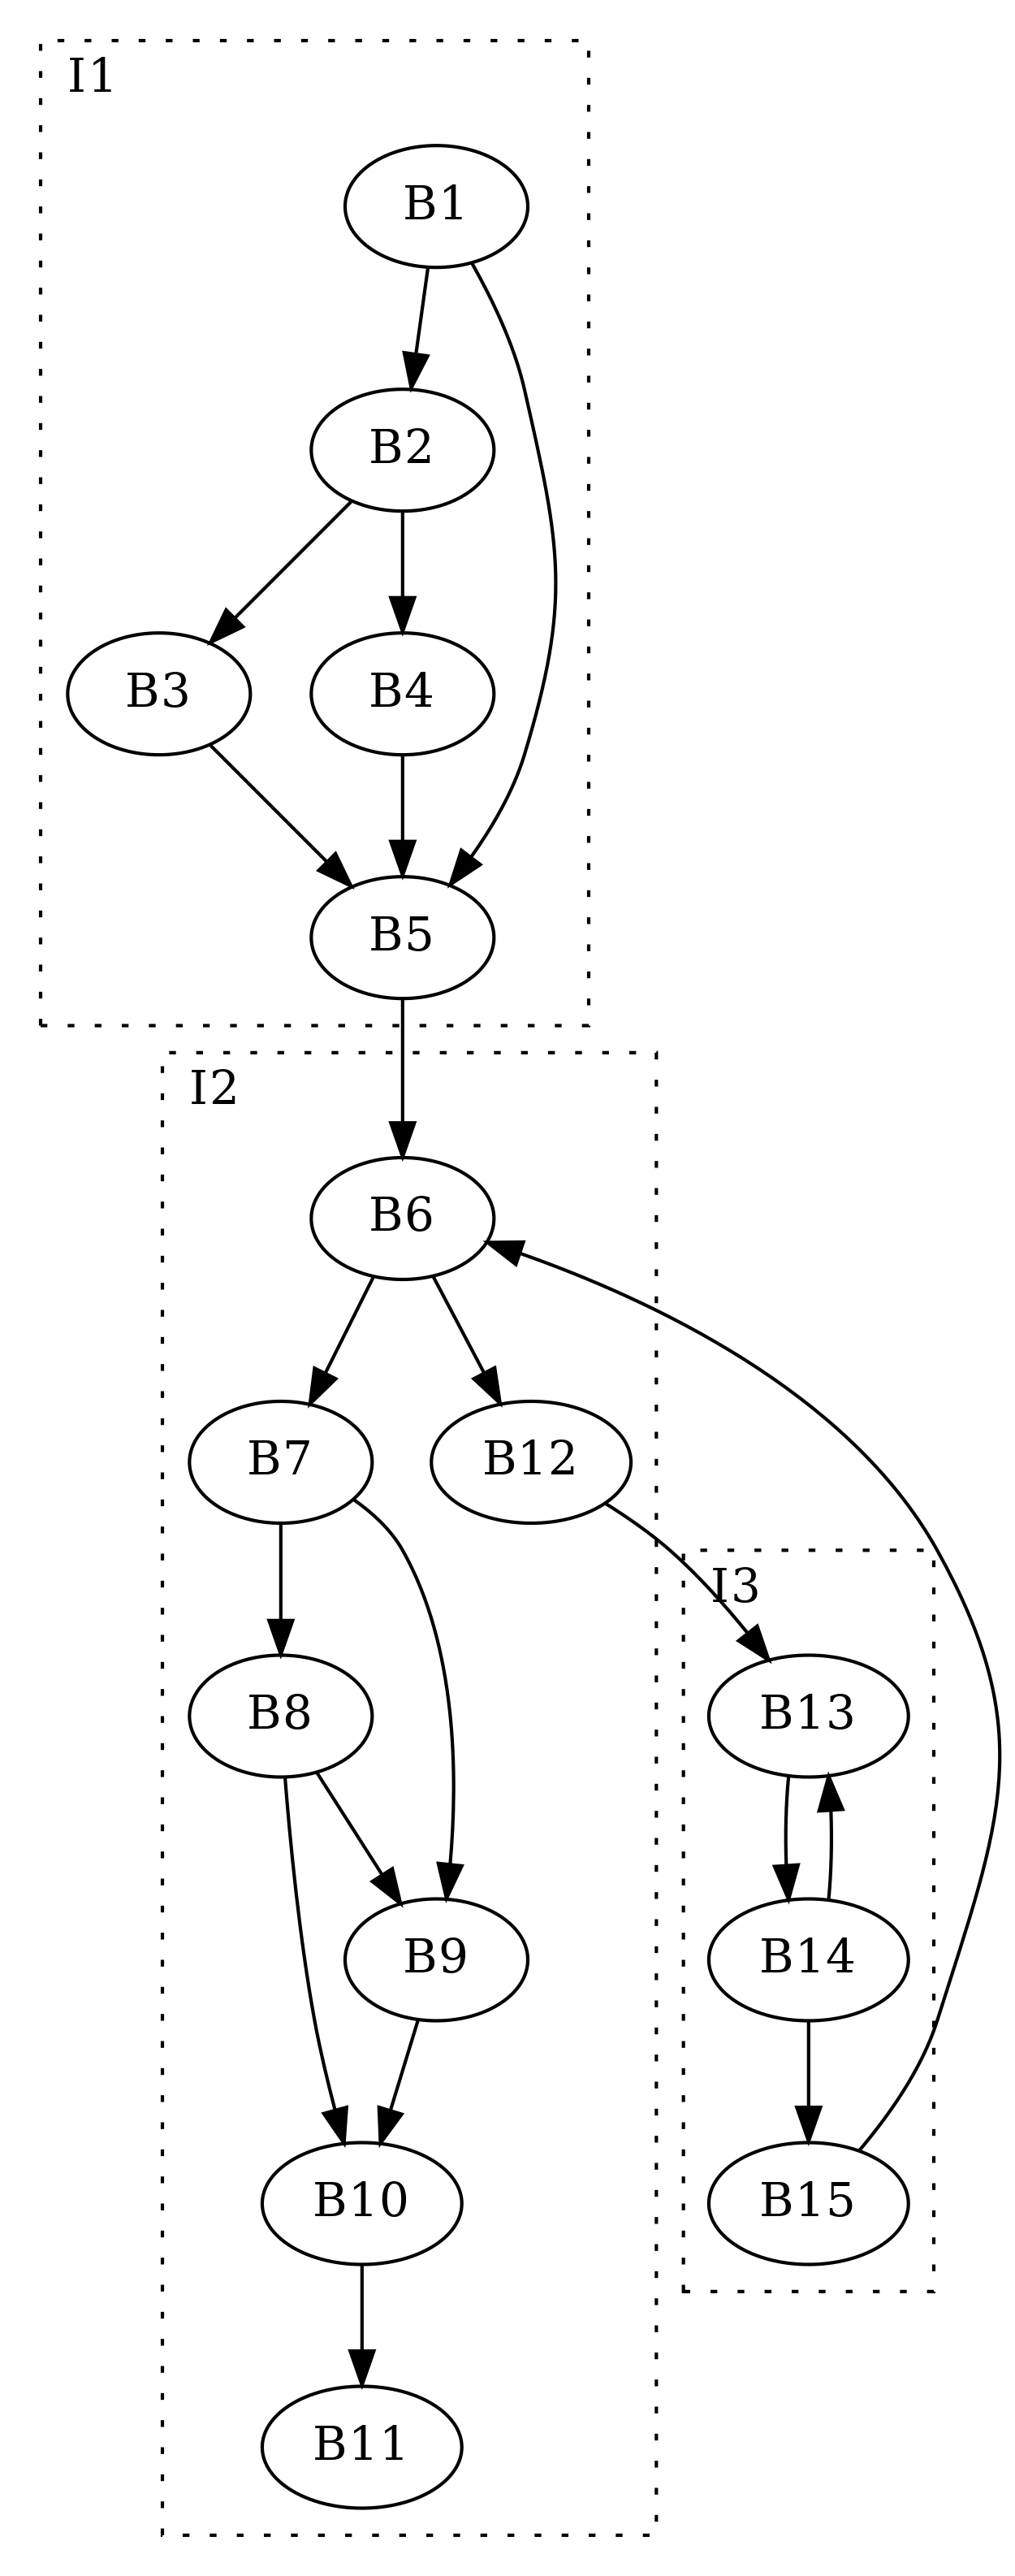
\includegraphics[width=\textwidth]{inc/methods/interval/G_1.png}
			\caption{$G^1$}
		\end{subfigure}
		\qquad
		\begin{subfigure}[b]{0.10\textwidth}
			\centering
			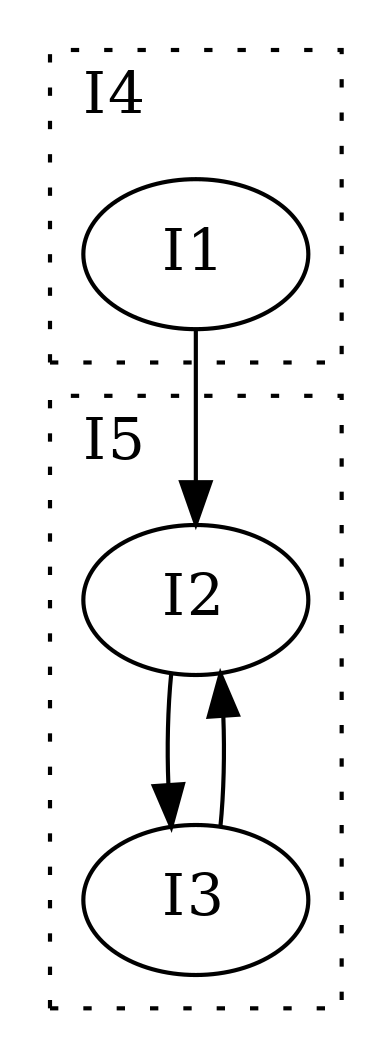
\includegraphics[width=\textwidth]{inc/methods/interval/G_2.png}
			\caption{$G^2$}
		\end{subfigure}
		\qquad
		\begin{subfigure}[b]{0.10\textwidth}
			\centering
			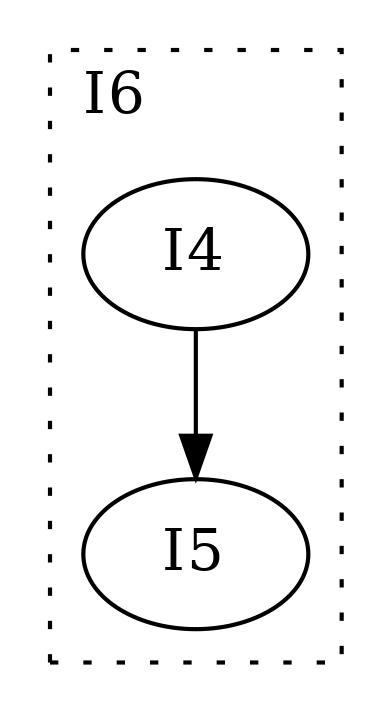
\includegraphics[width=\textwidth]{inc/methods/interval/G_3.png}
			\caption{$G^3$}
		\end{subfigure}
		\qquad
		\begin{subfigure}[b]{0.06\textwidth}
			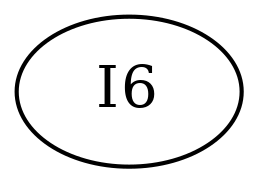
\includegraphics[width=\textwidth]{inc/methods/interval/G_4.png}
			\vspace{2em}
			\caption{$G^4$}
		\end{subfigure}
		\caption{Derived sequence of graphs, $G^1, ..., G^n$.}
	\end{figure}
\end{frame}

% ___ [ Interval - Example ] ___________________________________________________

\begin{frame}
	\frametitle{Interval method - example}

% TODO: One example for each method, how it works.
	TODO: add example for interval method.
\end{frame}

\begin{frame}
	\frametitle{Interval method - counter-example}

% TODO: One example for each method, counter-example when it doesn't work.
	TODO: add counter-example for interval method.

% Doesn't work when we have jump threading.
\end{frame}

% --- [ Pattern-independent method ] -------------------------------------------

\begin{frame}
	\frametitle{Pattern-independent method}

	Considers the conditions required to reach a node in the CFG rather than modelling explicit patterns. Relies on semantic-preserving transformations to pre-process CFGs.

	\vspace*{2em}

	\begin{block}{Pros}
		\begin{itemize}
			\item \textit{no} false negatives
			\item \texttt{goto}-free output
		\end{itemize}
	\end{block}

	\begin{block}{Cons}
		\begin{itemize}
			\item \textit{many} false positives
			\item introduces auxiliary condition variables (not present in original source)
		\end{itemize}
	\end{block}

% solved by pattern-independent method:

%    if (a & !b) {
%       // code1
%    }
%    if (b) {
%       // code 2
%    }
%    if (!b) {
%       // code 3
%    }

%    if (a & !b) {
%       // code1
%       goto LABEL_1
%    }
%    if (b) {
%       // code 2
%    }
%    if (!b) {
%    LABEL_1:
%       // code 3
%    }

\end{frame}

\begin{frame}
	\frametitle{Pattern-independent method}
	TODO: add reaching condition visualization.

	% TODO: add note about wrapping prog in endless-loop and adding condition can structure any program. Doesn't mean it's "right".
\end{frame}

% ___ [ Pattern-independent method - Example ] _________________________________

\begin{frame}
	\frametitle{Pattern-independent method - example}

% TODO: One example for each method, how it works.
	TODO: add example for patter-independent method.
\end{frame}

\begin{frame}
	\frametitle{Pattern-independent method - counter-example}

% TODO: One example for each method, counter-example when it doesn't work.
	TODO: add counter-example for patter-independent method.
\end{frame}

% === [ Technical Contributions ] ==============================================

\begin{frame}
	\frametitle{Technical Contributions}

% TODO: Description of what I did, and what I achieved.
	\begin{itemize}
		\item Give insight into how different control flow recovery method operate.
		\item Highlight the benefits and drawbacks of different control flow recovery methods -- so users may select the method best suited for their needs.
		\item Develop tools to facilitate an understanding of the inner workings of different control flow recovery methods.
		\item Provide intuition for deficiencies in control flow recovery methods, detailing their failure modes and giving insight to help guide future research.
		%\item Ultimately determine that there does not \textit{yet} exist a single control flow recovery method that outperforms all others with regards to false positive/false negative recovery and semantic equivalence.
	\end{itemize}

	%Build tools to help facilitate gaining an understanding of the inner workings of different control flow recovery methods.
	%and help facilitate a better understanding of the benefits and drawbacks of different control flow recovery methods.

\end{frame}

% === [ Future Work ] ==========================================================

\begin{frame}
	\frametitle{Future Work}

% TODO: speculations.

% The research community has developed three primary methods of control flow recovery (give or take), however, each method has deficiencies and distinguished strengths.

% TODO: Future work: the bullet points are too long to read

	\begin{itemize}
		\item Explore combining key principles from different control flow recovery methods to leverage their strengths and work around their deficiencies.
		\begin{itemize}
			\item Specifically, integrate knowledge from analysis using the Hammock method (which importantly has \textit{no false positives}) into the other methods, and provide a \textit{confidence score} to the recovered control flow primitives.
		\end{itemize}
		\item Explore leveraging control flow analysis results -- which enable high-level data flow analysis -- to improve upon binary analysis capabilities.
		\begin{itemize}
			\item Specifically, propagate data flow information into concolic execution engines to enable lifting of machine code with indirect branching instructions to LLVM IR. How to do this in a performant way is an open and active research topic.
		\end{itemize}
	\end{itemize}

% 2019-
%
% TODO: Summary of what happens in the academic community, main reserach happening.


\end{frame}

\begin{frame}
	\frametitle{Demo}

% Note to speaker: What you envision, would be the workflow to use a tool like that.

% Note to speaker: Would you automate it?
%    automate what you can prove to be correct.
%    manual intervention to disambiguate.
%    - what if you

Time for a demo!


\end{frame}

\end{document}
